\section{Story Diagrams} \label{sec:StoryDiagrams}

After explaining the concept of story patterns in Section~\ref{sec:StoryPatterns}, a prerequisite for this section, we explain the story diagrams themselves.
We give an overview of the general idea in Section~\ref{sec:IdeaStoryDiagrams} and go on with explaining the language constructs in the following sections.

\subsection{General Idea}\label{sec:IdeaStoryDiagrams}

% - combine activity diagrams and graph transformations as well as imperative, deterministic and declarative, non-deterministic languages to formally and compactly describe software behavior in terms of model transformations using an OO-based, familiar notation

The main idea behind story diagrams is to formalize UML activities
to better support model-driven software development.
This is done by not only modeling the software structure, but also completely modeling its behavior and, thus, making the software model executable.
For that purpose, graph transformations were chosen to formally specify behavior and have been combined with UML activities.
The result, story diagrams, is a mixture of two languages:
an imperative, deterministic language for the description of control flow, namely UML activities,
and a declarative, non-deterministic, object-oriented, graph-transformation-based language for the description of model modifications, so-called story patterns (see Section~\ref{sec:StoryPatterns}).
Both languages are graphical, formally defined, and use a familiar notation based on UML activities\footnote{Actually,
we use the notation of UML 1.5 activity diagrams, but already use the terminology of the UML 2.}
and UML object diagrams with minor modifications.

An exemplary story diagram is illustrated in Figure~\ref{fig:simpleStoryDiagram}.
This story diagram takes a graph-based representation (a model of a so-called abstract syntax graph, see Section~\ref{sec:typeGraph}) of an object-oriented program, e.g., in Java,
and replaces calls of a given method (\fe{oldMethod}) with calls of another given method (\fe{newMethod}).

\begin{figure}[htb]
  \centering
  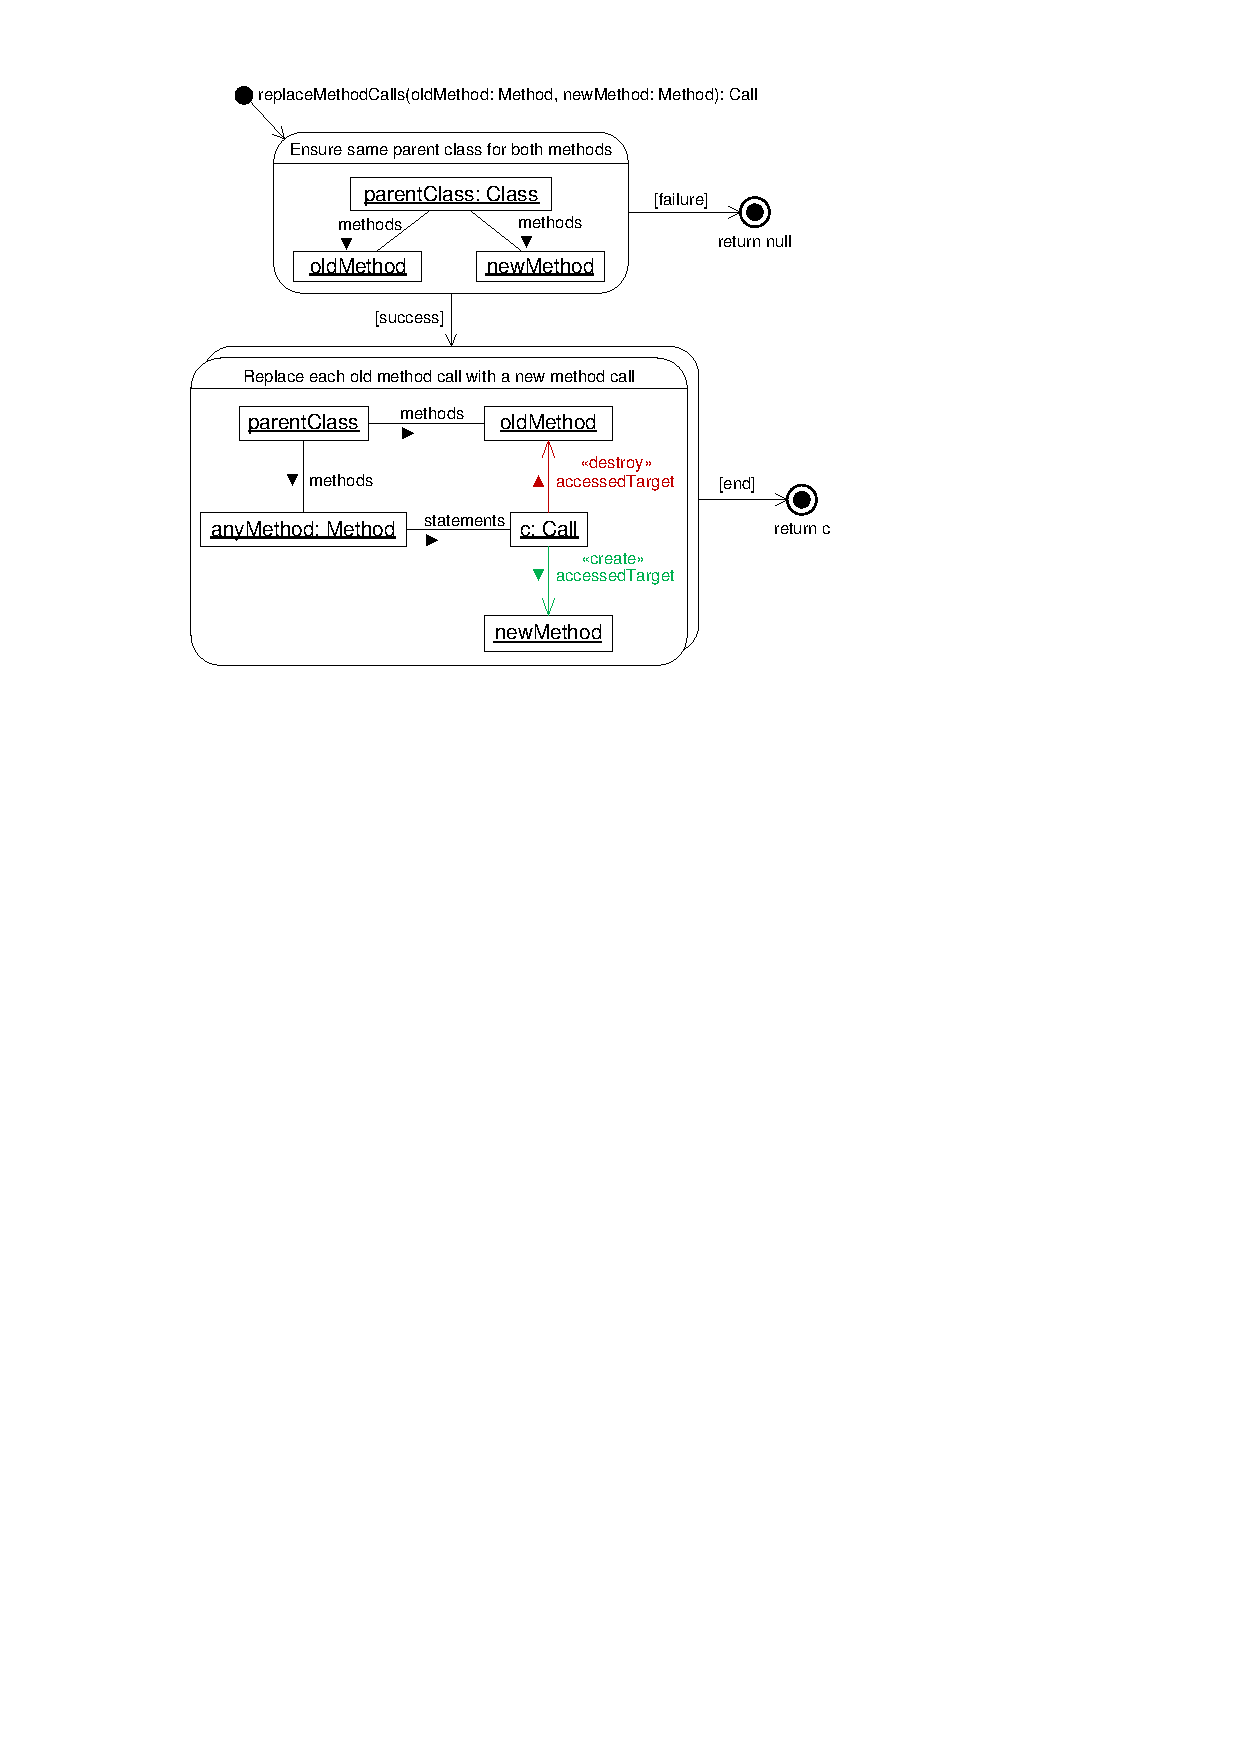
\includegraphics[scale=1.0]{figures/SimpleStoryDiagramExample}
  \caption{Exemplary Story Diagram -- Replace Method Calls}
  \label{fig:simpleStoryDiagram}
\end{figure}

Like UML activities, story diagrams model control flow by means of activity nodes and activity edges.
Each activity node embeds a story pattern to formally specify the behavior for this node\footnote{There are
some exceptions like activity call nodes which do not contain story patterns to specify the behavior.}.
The activity edges can carry guards.
These are either specified by boolean expressions, e.g., checking attribute values of a matched object,
or by keywords used to specify decisions on whether a story pattern could be
matched or not\footnote{A story pattern is successfully matched if for each object and link variable in the pattern corresponding objects and links are found in the instance model (host graph) and all specified constraints are satisfied.}.
In Figure~\ref{fig:simpleStoryDiagram}, the used guards are \fe{\text[success\text]} (successful execution of a story pattern),
\fe{\text[failure\text]} (failed to completely execute a story pattern),
and \fe{\text[end\text]} (activity edge points to the first activity node to be executed after a loop).

In contrast to ordinary UML activities, story diagrams, so far, do not model concurrent execution.
Thus, the language constructs \emph{fork} and \emph{join} are currently not supported in story diagrams.
We plan to include these concepts in future versions of story diagrams.

%- Story diagrams in MDSD process, 2 worlds: stand-alone transformations and specifications of methods' behavior:
%  1. alternative (completely modeling software): model classes in class diagrams, specify their methods' behavior in story diagrams, generate executable source code (e.g. Java) or use an interpreter
%  2. alternative (specify recurring model operations/transformations for a given type of models): model only classes representing the editor's model under development (meta-model), specify modification operations of this model (adding and removing elements, analysis operations, translations to/generation of other models, etc.), need of a software that triggers the specified operations, the operations can be performed using generated code or an interpreter
%- introduce an example

Basically, there are two different ways of using story diagrams in a model-driven software development process.

Originally, story diagrams were used in object-oriented software development to formally specify the behavior of methods that are defined in classes.
Calling such a method means to execute the story diagram that represents the method's behavior.
If there is a story diagram that models the behavior for each method specified in a class model,
the software model completely covers the software's structure and behavior and, thus, can be analyzed and executed.
In this case, story diagrams specify the behavior of objects whose properties are defined by classes.
For that reason, those story diagrams have a \emph{this} variable -- similar to the keyword \emph{this} in Java -- representing the object (a class instance) that they belong to (a self reference).
This variable can be used as a starting point for the graph matching specified in a story diagram.

For example, the class diagram in Figure~\ref{fig:SDWithThisClassDiagram} defines a method \fe{findAttribute} for all \fe{Class} objects.
This method's behavior is specified by the story diagram in Figure~\ref{fig:SDWithThis}.
The matching of the object structure specified in the contained story pattern, in this case,
starts with the \fe{this} object variable of the type \fe{Class} which is already bound
to the \fe{Class} object that the \fe{findAttribute} method belongs to.
Thus, this method tries to find an attribute \fe{a} in the same class with the name given by the method's parameter \fe{text}.

\begin{figure}[htb]
	\centering
  \begin{minipage}[t]{.4\textwidth}
    \centering
    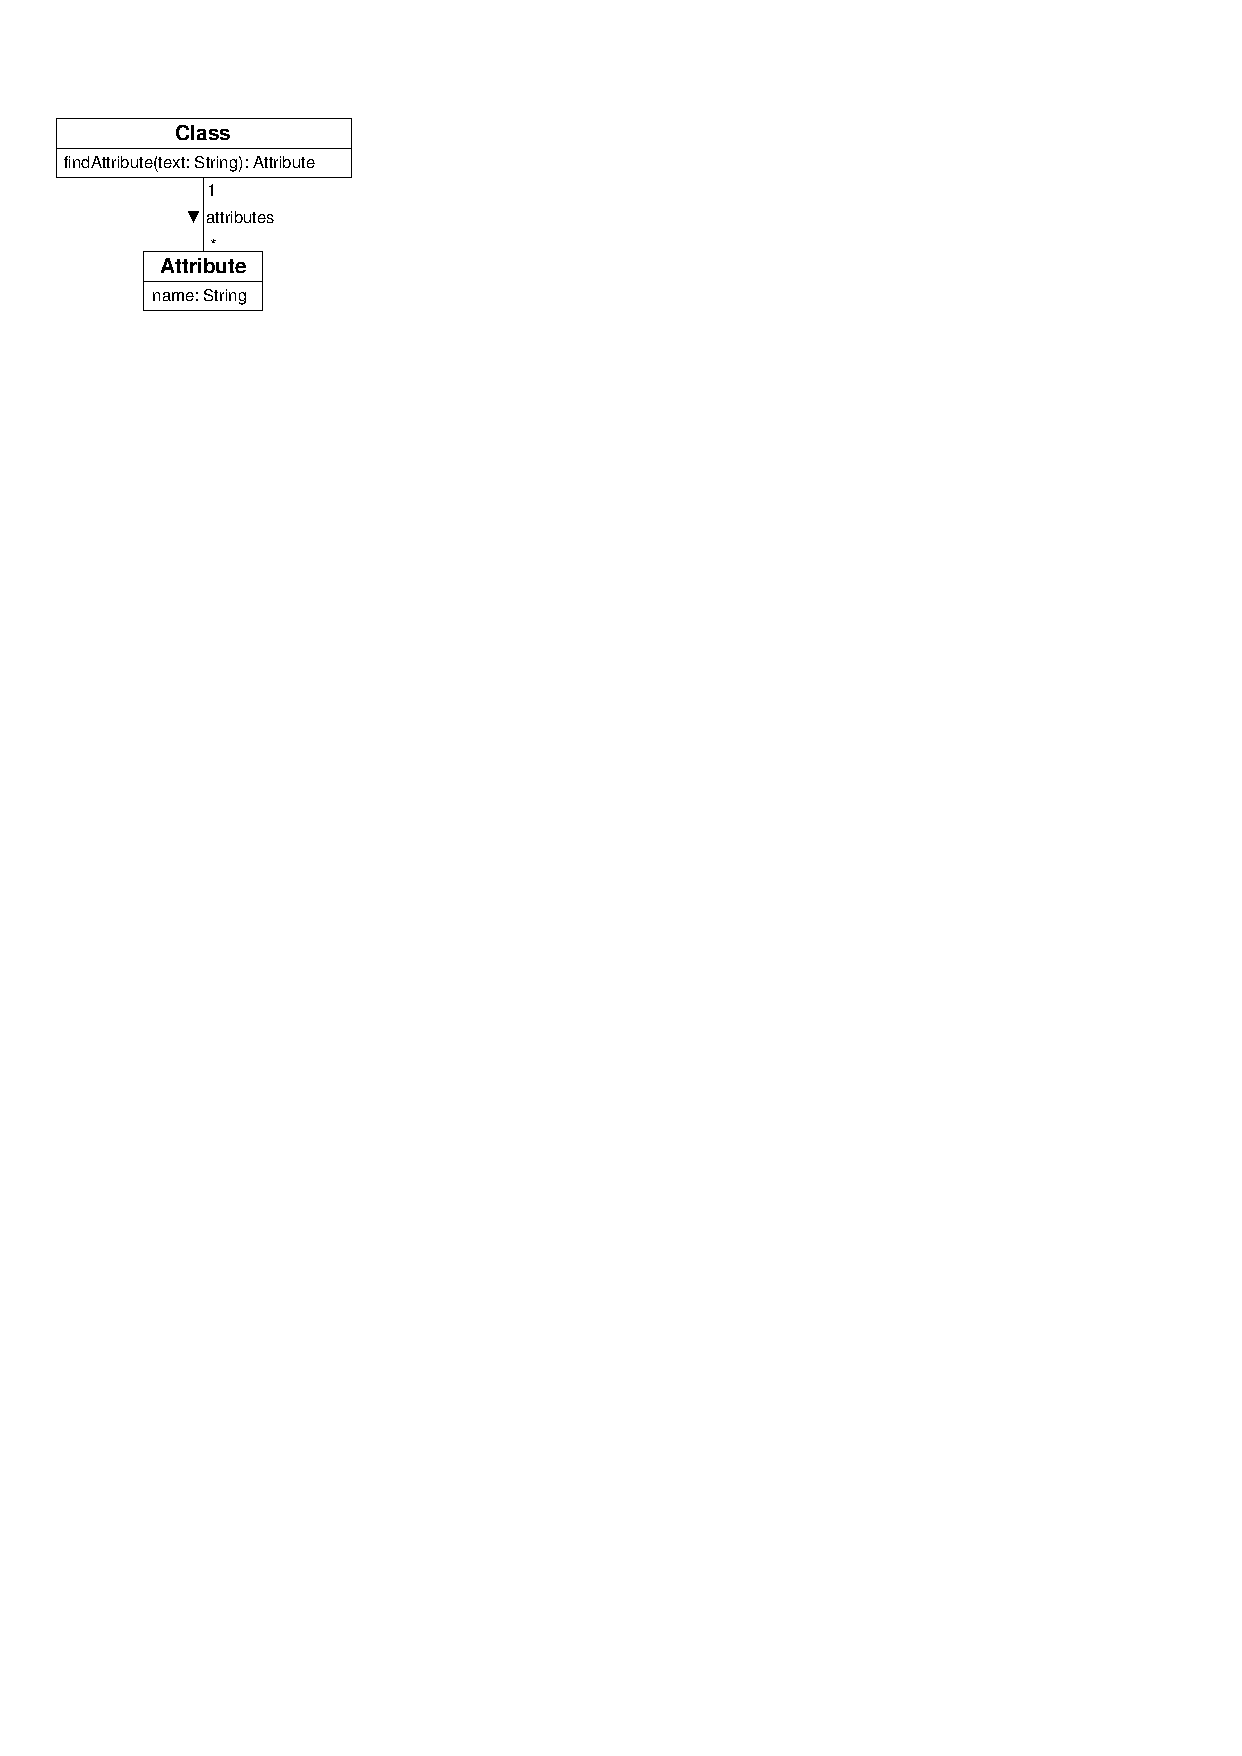
\includegraphics[scale=1]{SimpleSDFindAttributeClassDiagram} 
    \caption{Type Model for the Story Diagram in Figure~\ref{fig:SDWithThis}}
    \label{fig:SDWithThisClassDiagram}
  \end{minipage}%
  \hfill
  \begin{minipage}[t]{.55\textwidth}
    \centering
    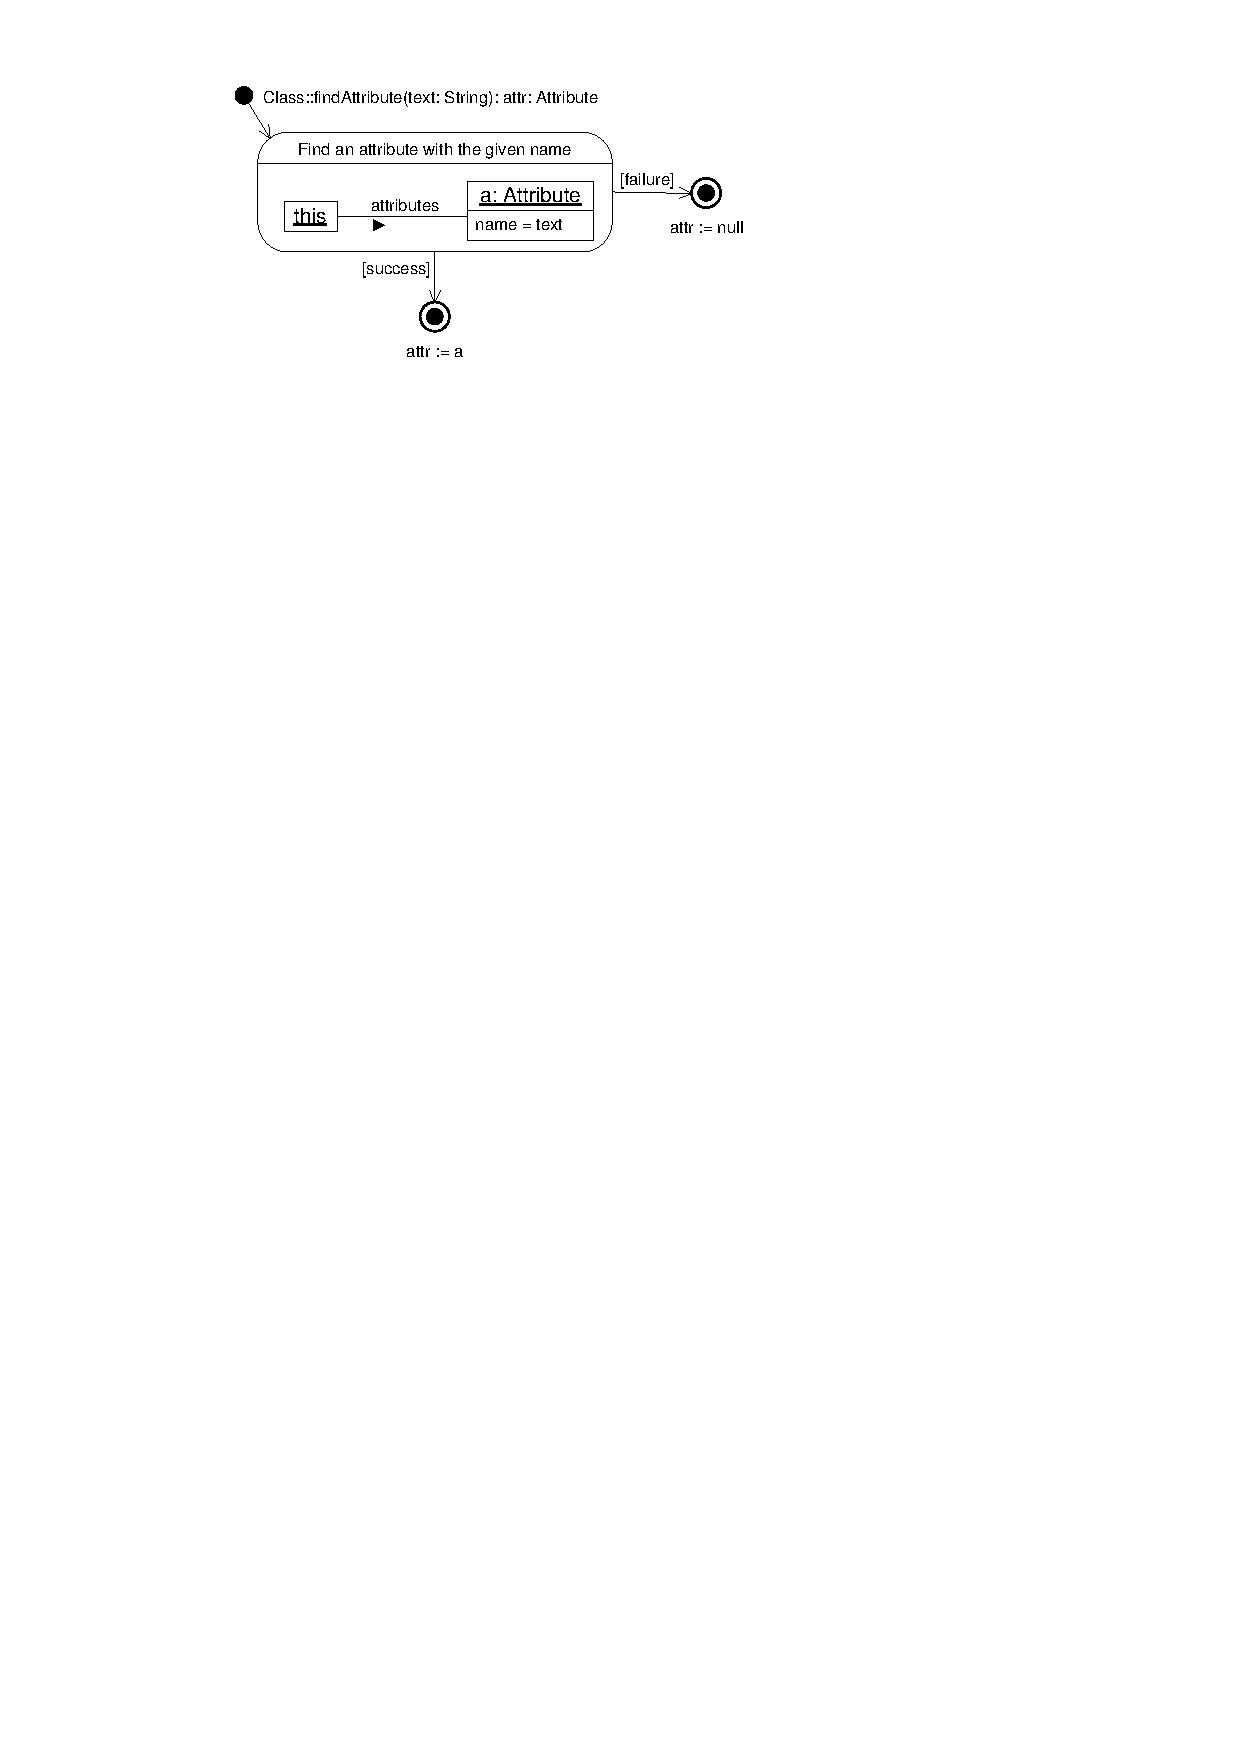
\includegraphics[scale=1]{SimpleSDFindAttribute}
    \caption{Exemplary Story Diagram With \emph{this} Object Variable}
    \label{fig:SDWithThis}
  \end{minipage}
\end{figure}

\begin{figure}[htb]
	\centering
  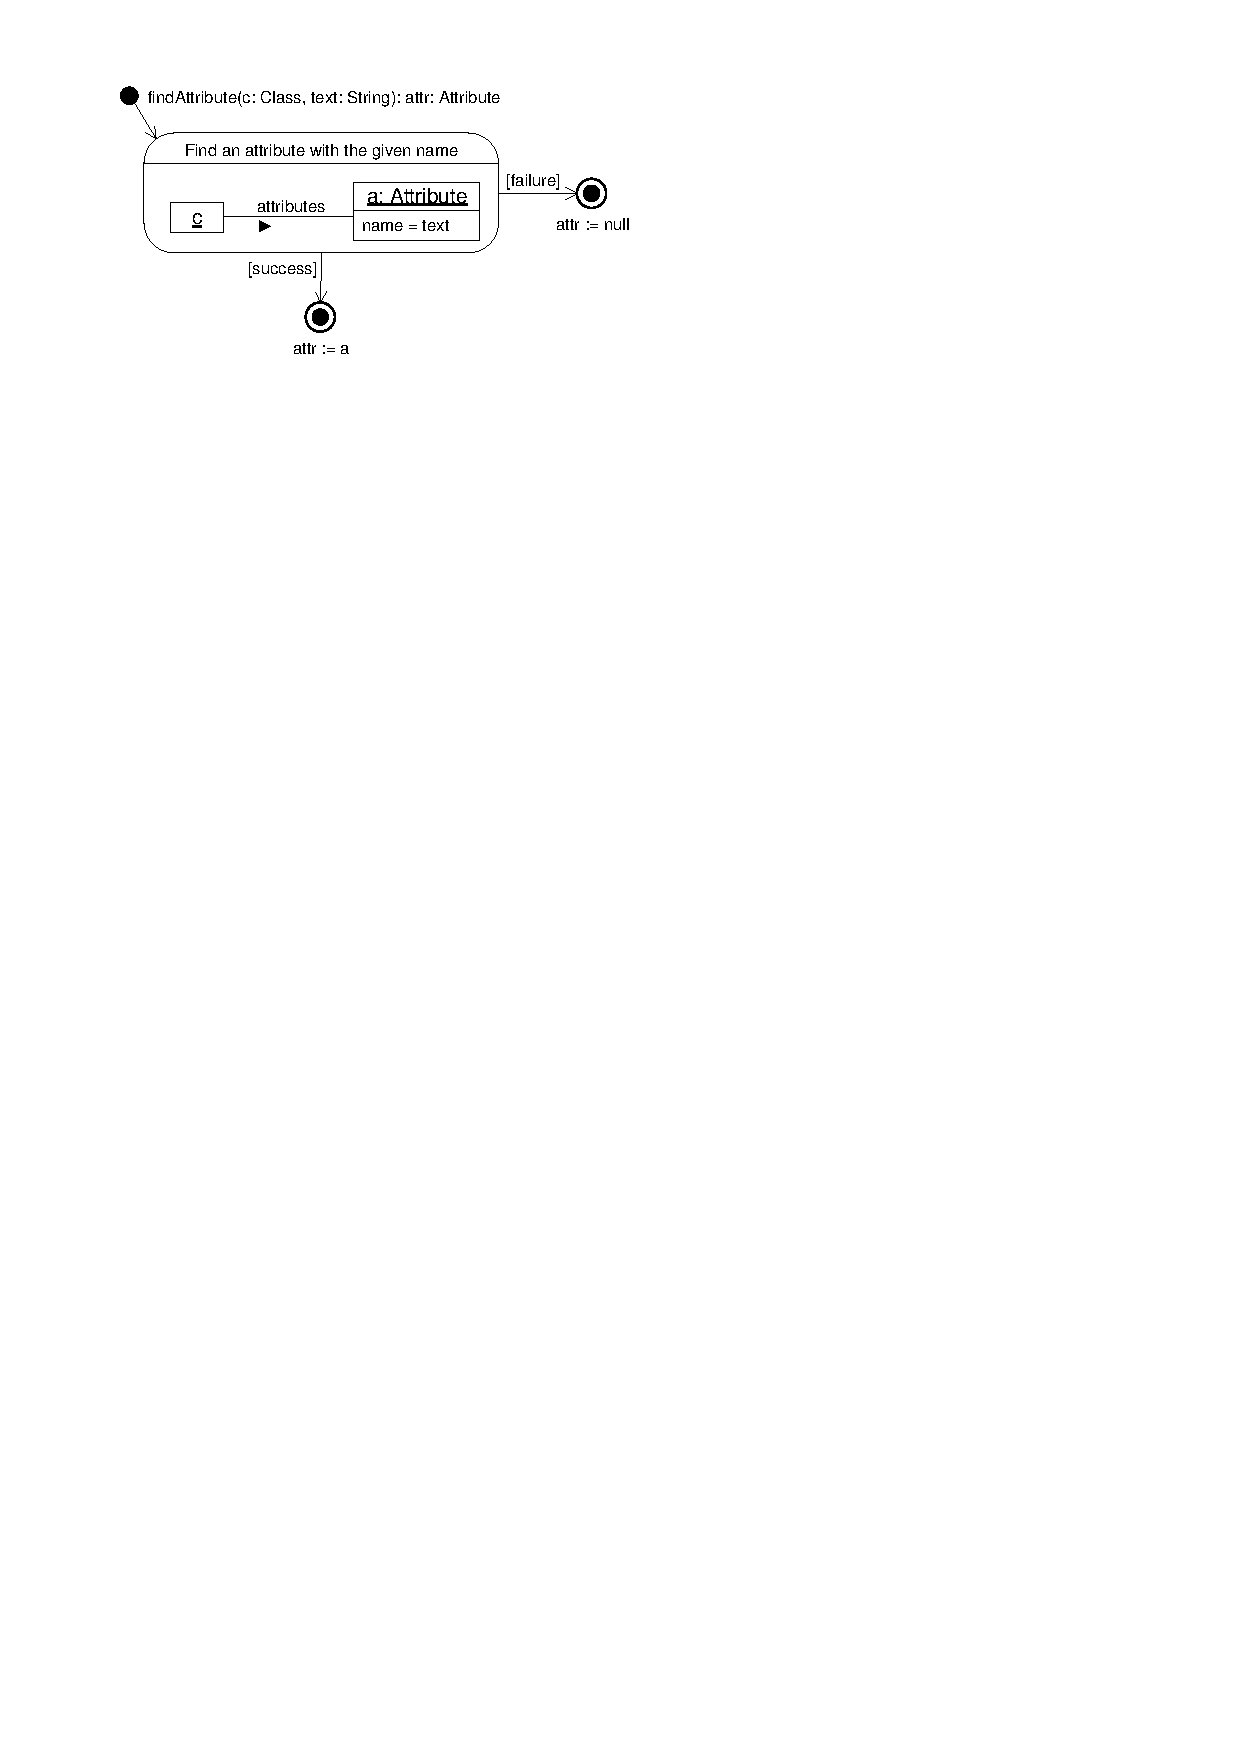
\includegraphics[scale=1]{SimpleSDFindAttributeStatic} 
  \caption{Exemplary Story Diagram Without \emph{this} Object Variable}
  \label{fig:SDWithThisStatic}
\end{figure}

Another more flexible way of using story diagrams is to specify any kind of model transformation or operation in a story diagram without attaching this behavior to a certain class.
In contrast to the previous case, there is no \emph{this} variable that could be used as a starting point for the graph matching.
All starting nodes for the graph matching have to be provided as arguments of the story diagram call.
For this purpose, in contrast to the story diagram in Figure~\ref{fig:SDWithThis}, the story diagram in Figure~\ref{fig:SDWithThisStatic} has an additional parameter \fe{c}.
The corresponding arguments of a story diagram call are assumed to be known (bound object variables) and are used as starting points for the graph matching.
This way, the operations or transformations defined by story diagrams can be used from within any other part of the developed software, like a software library would be used.
Typically, model-to-model transformations, consistency checks, or more generally speaking, recurring and object-independent operations are defined this way.

% - enable formal analyses to check/ensure certain behavioral software properties

In both cases, story diagrams can be used to generate executable source code or be executed using an interpreter.
Besides execution, the formally defined story diagrams can also be analyzed to guarantee certain behavioral properties \cite{Mey09,Zue09}.
For example, model checking can be used to check whether a certain invariant holds
(e.g.\ that all accessible variables are still accessible after a refactoring operation)
or if a critical state can ever be reached (e.g.\ if an attribute or method has no parent class after a refactoring operation which would result in an incorrect program).

A complete description of the story diagrams' abstract syntax is given in the Appendix~\ref{sec-reference}.
There is also a grammar that determines all feasible story diagrams by constraining their structure.
The latest version of this grammar can be found in Thomas Klein's diploma thesis \cite{Kle99}.


%\subsection{The Language Constructs in Story Diagrams (Jan/Dietrich)}\label{sec:StoryDiagrams:composition}

\subsection{Activities, Activity Parameters and Return Values}\label{sec:activities}

Since story diagrams can be seen as special UML activities, we reused the class names defined by the UML 2.
Thus, similar to UML activities, a story diagram is represented by a so-called activity (class \fe{Activity}).

Each story diagram can have parameters.
We distinguish \emph{in} and \emph{out} parameters,
i.e.\ parameters representing arguments given when a story diagram is called (\emph{in})
and parameters representing return values (\emph{out}).
Parameters are either \emph{in} or \emph{out} parameters.
%Parameters can be \emph{in} and \emph{out} parameters at the same time.
The story diagram in Figure~\ref{fig:SDWithThisStatic} has two \emph{in} parameters \fe{c} and \fe{text}
as well as an \emph{out} parameter \fe{attr} of the type \fe{Attribute}.
If there are more than one \emph{out} parameter, these are comma-separated.

If a story diagram defines the behavior of a method, the parameters are defined by the corresponding method's signature.
In this case, the number of \emph{out} parameters is limited to one single parameter and represents the only \emph{return} value of the method and story diagram.
Besides these parameters, there is another implicitly defined parameter \fe{this}
which -- similar to Java's \fe{this} keyword -- represents the object that the story diagram belongs to.

In case a story diagram is not defining a method's behavior, it defines its own signature explicitly with according \emph{in} and \emph{out} parameters.
The number of \emph{out} parameters is allowed to be arbitrary in this case and there is no \emph{this} parameter.

The values or objects returned after execution of a story diagram are defined by expressions in the \emph{stop} activity nodes.
For example, the object matched to the object variable \fe{a} is returned by the story diagram in Figure~\ref{fig:SDWithThisStatic} in case of a successful execution.
This is specified by the expression \fe{attr := a} which represents an assignment of the value of object variable \fe{a} to the \emph{out} parameter \fe{attr}.
Otherwise, an empty reference is returned which is specified by the keyword \fe{null}.
This notation is taken from Matthias Meyer \cite{Mey09}.

\subsection{Activity Nodes, Activity Edges} 
\label{sec:storydiagrams:activitynodes}

A story diagram's control flow is defined by activity nodes and activity edges, similar to UML activities.
Except for the cases where an activity node represents a call of another story diagram,
each node embeds a story pattern to specify the corresponding behavior.
Such activity nodes are called \emph{story nodes}.
Executing a story node results in executing the embedded story pattern.

In contrast to single story patterns, story patterns contained in story nodes of a story diagram have a different scope.
Here, you can reuse all object variables declared in the story patterns of preceding story nodes.
For example, in Figure~\ref{fig:simpleStoryDiagram} (p.~\pageref{fig:simpleStoryDiagram}),
the object variable \fe{parentClass} is reused in the second story pattern
by specifying the variable as a bound variable, i.e.\ the variable does not have to be matched anymore.

Executing a story node means executing the corresponding story pattern
which, in turn, means finding a subgraph with the specified properties
(e.g.\ finding objects of a certain type, with certain attribute values, and with certain connections)
and performing specified modifications of the found subgraph
(e.g.\ creating or removing objects and links or changing their attribute values).

We distinguish two kinds of story nodes: \emph{modifying story nodes} and \emph{matching story nodes}.
A matching story node contains a story pattern that only matches a specified object structure, but does not change it.
A modifying story node also performs modifications of the matched object structure.
For static analyses of model transformations described with story diagrams,
it is helpful to know which transformations do not modify the instance model.

\subsection{Activity Final Nodes} \label{sec:StopNodes}

The application of a story diagram can succeed or fail.
Usually, when the matchings are successful and the specified transformations can be carried out, the story diagram is considered to be applied successfully.
When a matching is unsuccessful somewhere or something unforeseen happens and the application has to be aborted, the story diagram's application is considered to have failed.
This is comparable to a method call either returning a desired result or returning false or null if something goes wrong.

\tododt{I would remove or replace this first paragraph.
In my opinion, the success and failure of story diagrams are not necessarily dependent on the success or failure of some pattern matchings or transformations in the same story diagram.
In Figure~\ref{fig:successAndFailureStopNodes} one could also model that the story diagram is considered to be successfully executed if the matching in the first story pattern fails.
Thus, success or failure of a story diagram is used like an implicitly declared boolean out parameter describing if the operation described by a story diagram is considered to be successful.
In which case it is successful is specified by the developer, not by the story diagrams language.
I would point out that the success of a story diagram is not directly dependent on the successful execution of all contained story patterns.
In contrast, the success and failure of story patterns are defined by the language.}

When one story diagram calls another, the calling story diagram's further execution may depend on the called story diagram's application being successful.
For example, the calling story diagram might need a return value of the called story diagram or it may only continue in a meaningful way if the called transformation has succeeded.
Therefore, a means to express and communicate the successful or unsuccessful application of a story diagram is required.
Story diagrams have success and failure final nodes for this.

In normal UML activities, the final nodes determine where control flow of the activity ends.
Story diagrams reuse this concept but they annotate the nodes with either \emph{success} or \emph{failure}.
Figure~\ref{fig:successAndFailureStopNodes} shows and example.

\begin{figure}[htb]
\begin{center}
  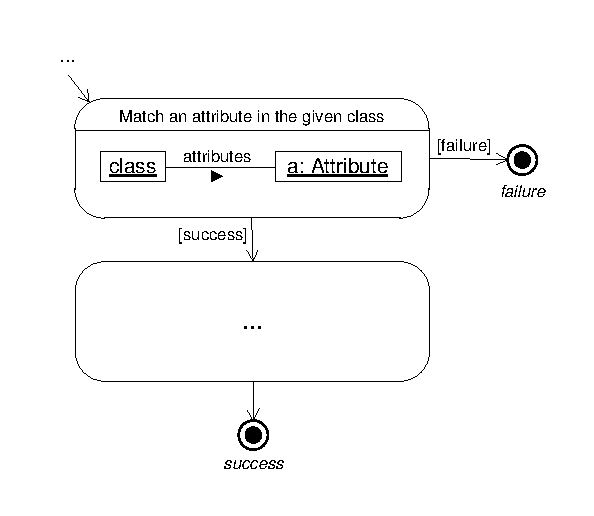
\includegraphics[width=0.7\textwidth]{figures/SuccessAndFailureStopNodes}
  \caption{Example of a success and a failure final node.}
  \label{fig:successAndFailureStopNodes}
\end{center}
\end{figure}

The upper story node in Figure~\ref{fig:successAndFailureStopNodes} specifies that an attribute of a given class object should be matched.
The failure activity edge leads to a final node also labelled with \emph{failure}.
This indicates that the application of the story diagram went wrong.

If an attribute object can be matched however, the control flow continues via the success activity edge to another story node.
Finally, it reaches a final node labelled with \emph{success}.
This indicates that the story diagram's application is considered to be successful.

While the execution of a story diagram is aborted upon reaching a failure final node, the effects of the execution up to this point are not reversed.
All modifications, e.g., object creations and deletions persist.
The developer of a story diagram has to keep this in mind when specifying a transformation.
If these side effects of failed story diagram applications are undesired, the story diagram has to be designed such that it is only aborted if no modifications already took place.
Another way would be to explicitly specify activity nodes which undo the modifications before going to the failure final node.

\todomvd{We could think about a rollback mechanism for later versions.}

\todomvd{Write something about the technical side of the propagation?}
\todoall{Modify metamodel accordingly.}

\subsection{Decision Nodes, Guards, and Loops}
\label{sec:DecisionNodesEtc}

The behavior of a story node is defined by its story pattern.
Therefore,
since trying to find a subgraph defined by a story pattern can fail,
each execution of a story node can also fail.
\tododt{Where is the meaning of failure described exactly? Should it be here or in the story patterns section?
Does success of a story pattern execution mean that there was a successful matching only, independly of the succeeding transformations,
or does it mean that the graph transformation (if available) could also be executed (was executable without contradictions, exceptions not considered)?
I think, success should include the transformation and we should, if possible, check
if a modifying story pattern can perform its modifications after a successful matching \emph{before} actually modifying the host graph
(check if all variables are matched and if there are contradictions).
Someone has to describe that in the story patterns section or here.}

To distinguish the cases of a successful story node execution and its failure,
the outgoing activity edges can be provided with the guards \fe{\text[success\text]} and \fe{\text[failure\text]} (see Figure~\ref{fig:SD-decisions} a)).
The control flow is following the activity edge with the \emph{success} guard in case of a successful story node execution,
i.e.\ a successful matching of the corresponding story pattern.
Otherwise it follows the activity edge with the \emph{failure} guard.
If an outgoing activity edge has no guard, it covers both cases, success and failure.
The guards \fe{\text[success\text]} and \fe{\text[failure\text]} can only be used pair-wise (exactly two outgoing activity edges with exactly these two guards).
The first story node in Figure~\ref{fig:simpleStoryDiagram} (p.~\pageref{fig:simpleStoryDiagram}), for example, uses these guards.

\begin{figure}[htb]
	\centering
  \begin{minipage}[t]{.5\textwidth}
    \centering
    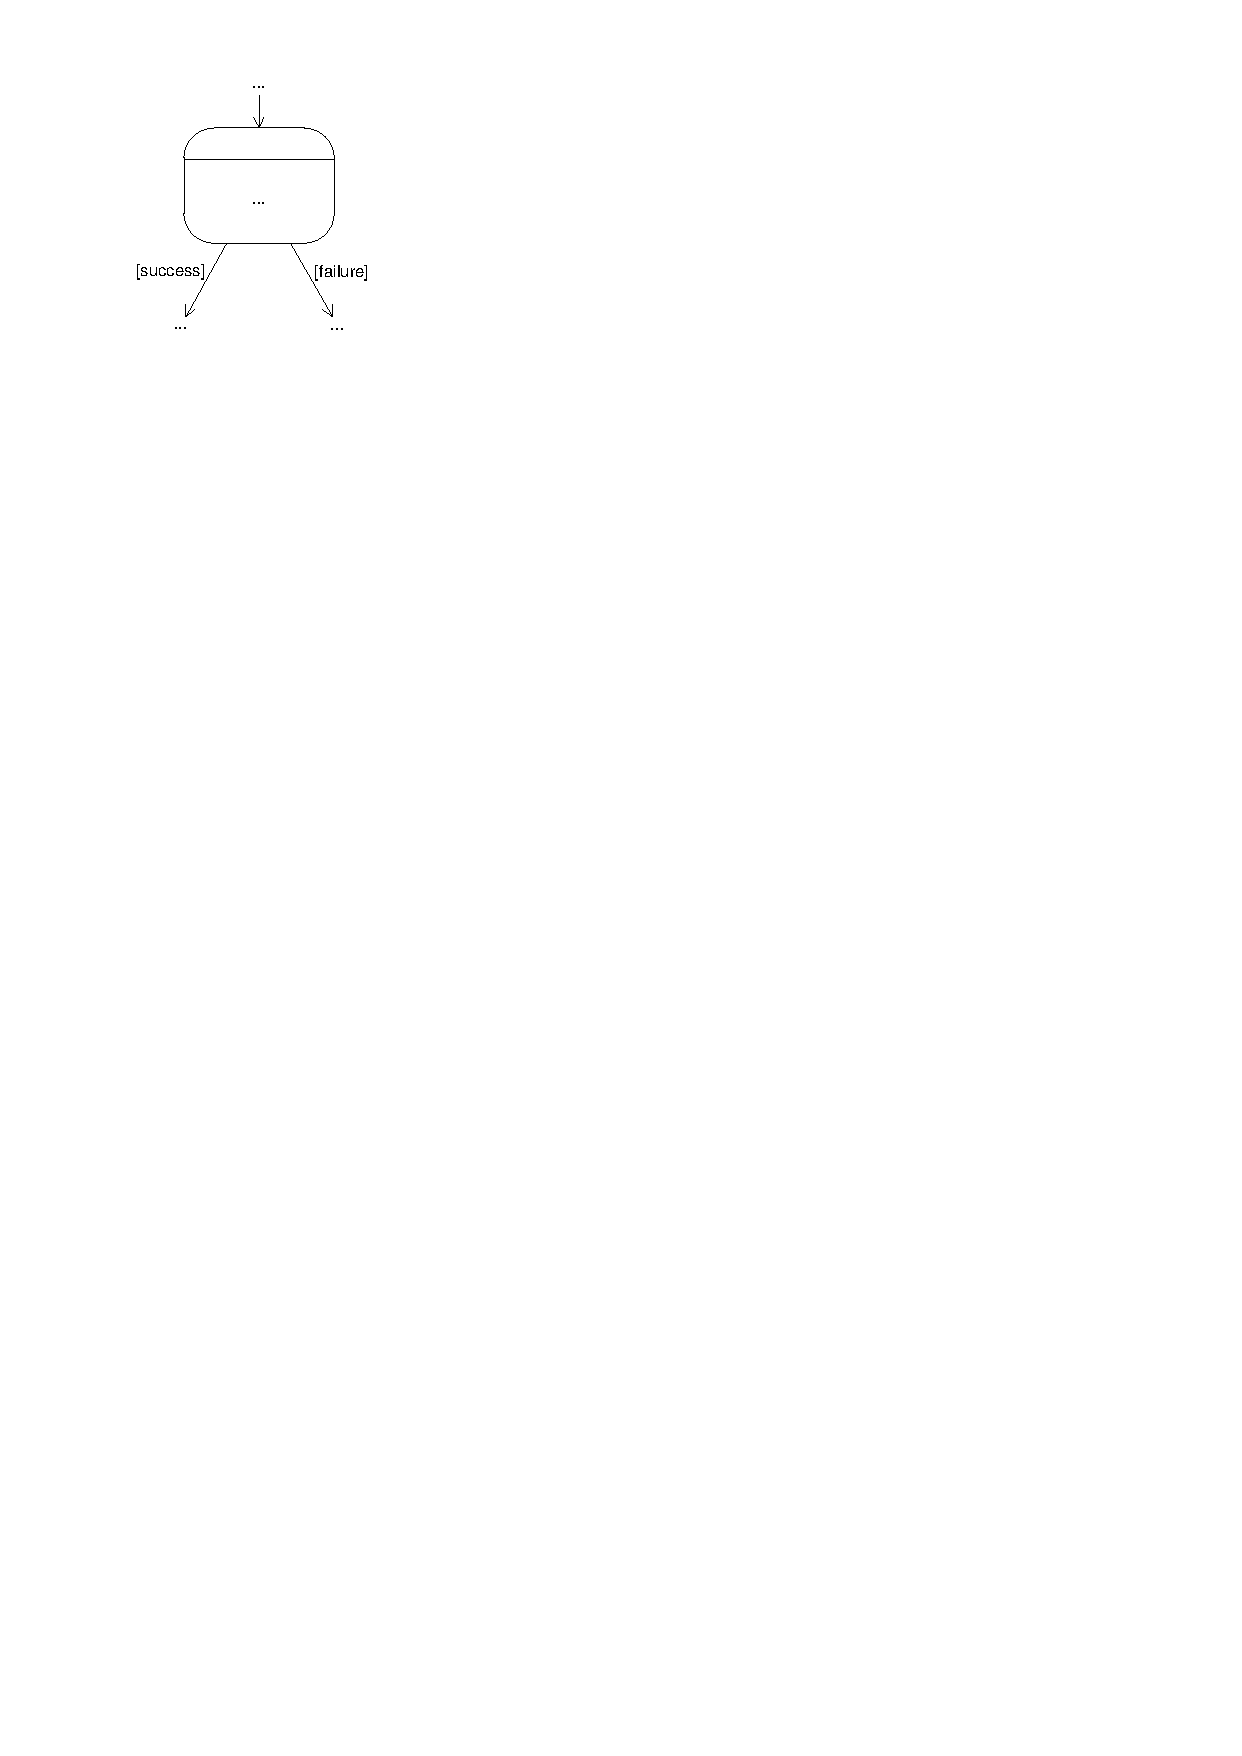
\includegraphics[scale=1]{SD-decision1}
    \\a)
    %\caption{a) Matching-Dependent Decision}
    %\label{fig:SD-decision-success}
  \end{minipage}%
  \hfill
  \begin{minipage}[t]{.5\textwidth}
    \centering
    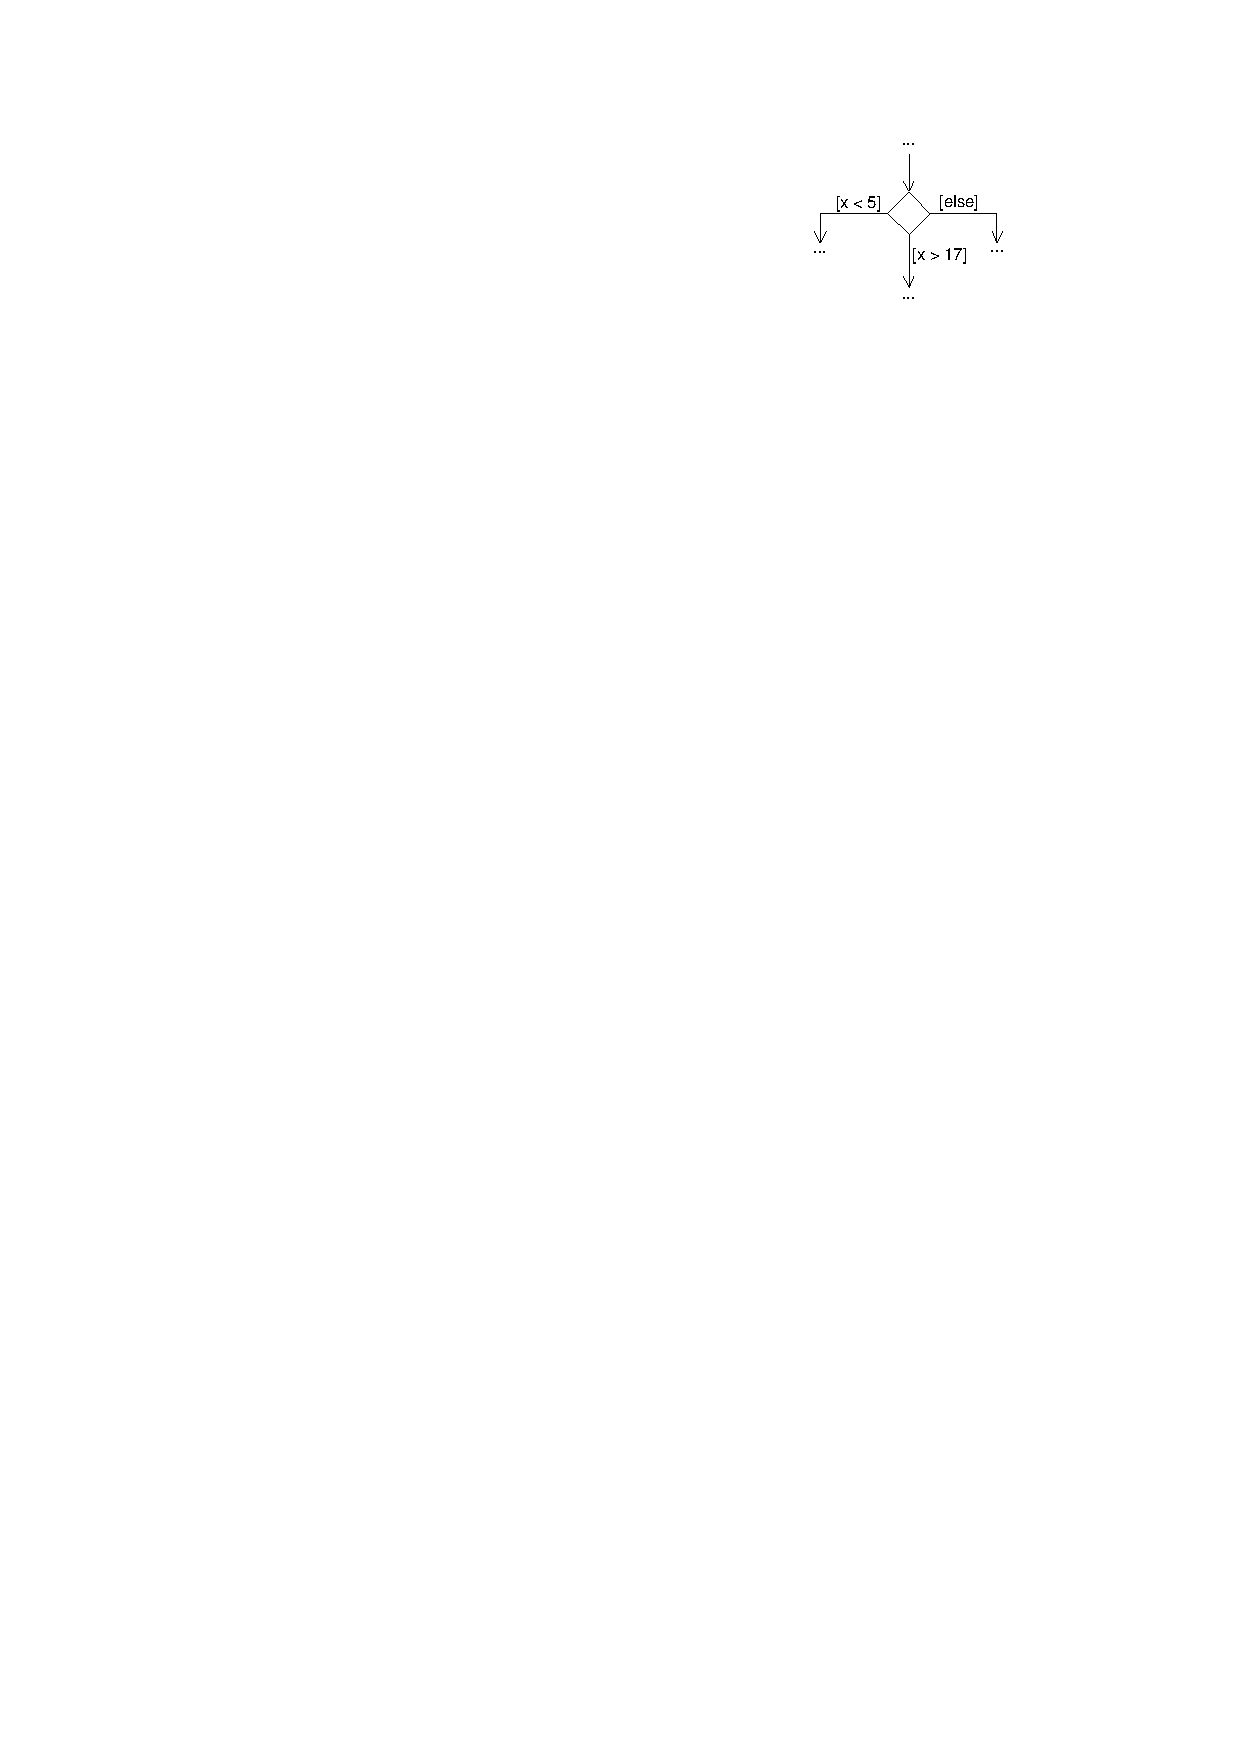
\includegraphics[scale=1]{SD-decision3}
    \\b)
    %\caption{b) Decision Node}
    %\label{fig:SD-decision-boolean}
  \end{minipage}
%  \hfill
%  \begin{minipage}[t]{.3\textwidth}
%    \centering
%    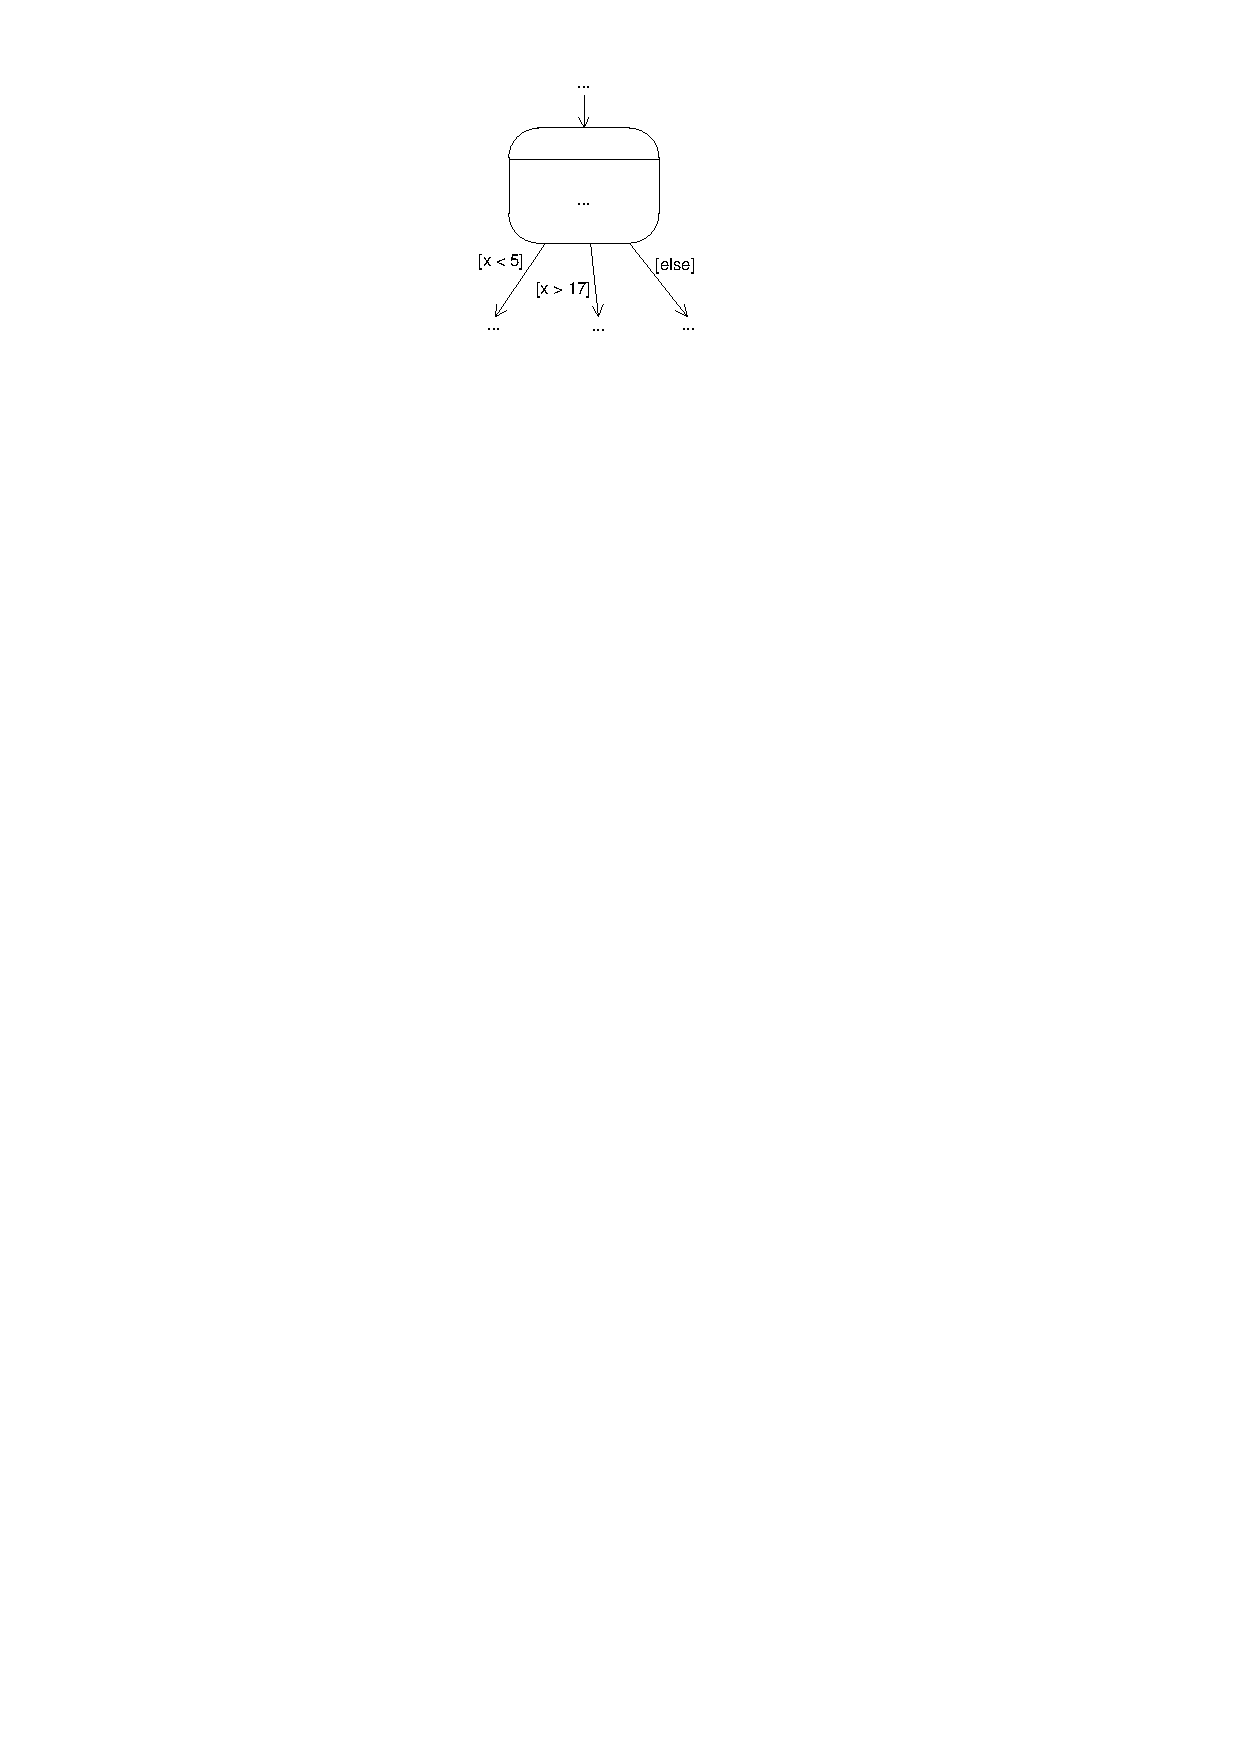
\includegraphics[scale=1]{SD-decision2}
%    \\c)
%    %\caption{c) Boolean Conditions}
%    %\label{fig:SD-decision-nodes}
%  \end{minipage}
  \caption{Examples For Decisions}
  \label{fig:SD-decisions}
\end{figure}

Besides \fe{\text[success\text]} and \fe{\text[failure\text]}, boolean expressions can be used as guards (see Figure~\ref{fig:SD-decisions} b)).
We use the \emph{junction node} -- depicted as a diamond -- for decisions that do not depend on a previous story node.
In this case, the boolean expression of the outgoing activity edge is evaluated to \emph{true} or \emph{false}.
There can be arbitrarily many outgoing activity edges with boolean guard expressions.
The boolean expressions have to mutually exclude each other
and the corresponding guards have to be combined with an outgoing activity edge with the guard \fe{\text[else\text]}.
I.e., if there is a guard with a boolean expression, there is also an activity edge with the guard \fe{\text[else\text]}.

\begin{figure}[htb]
	\centering
  \begin{minipage}[t]{.24\textwidth}
    \centering
    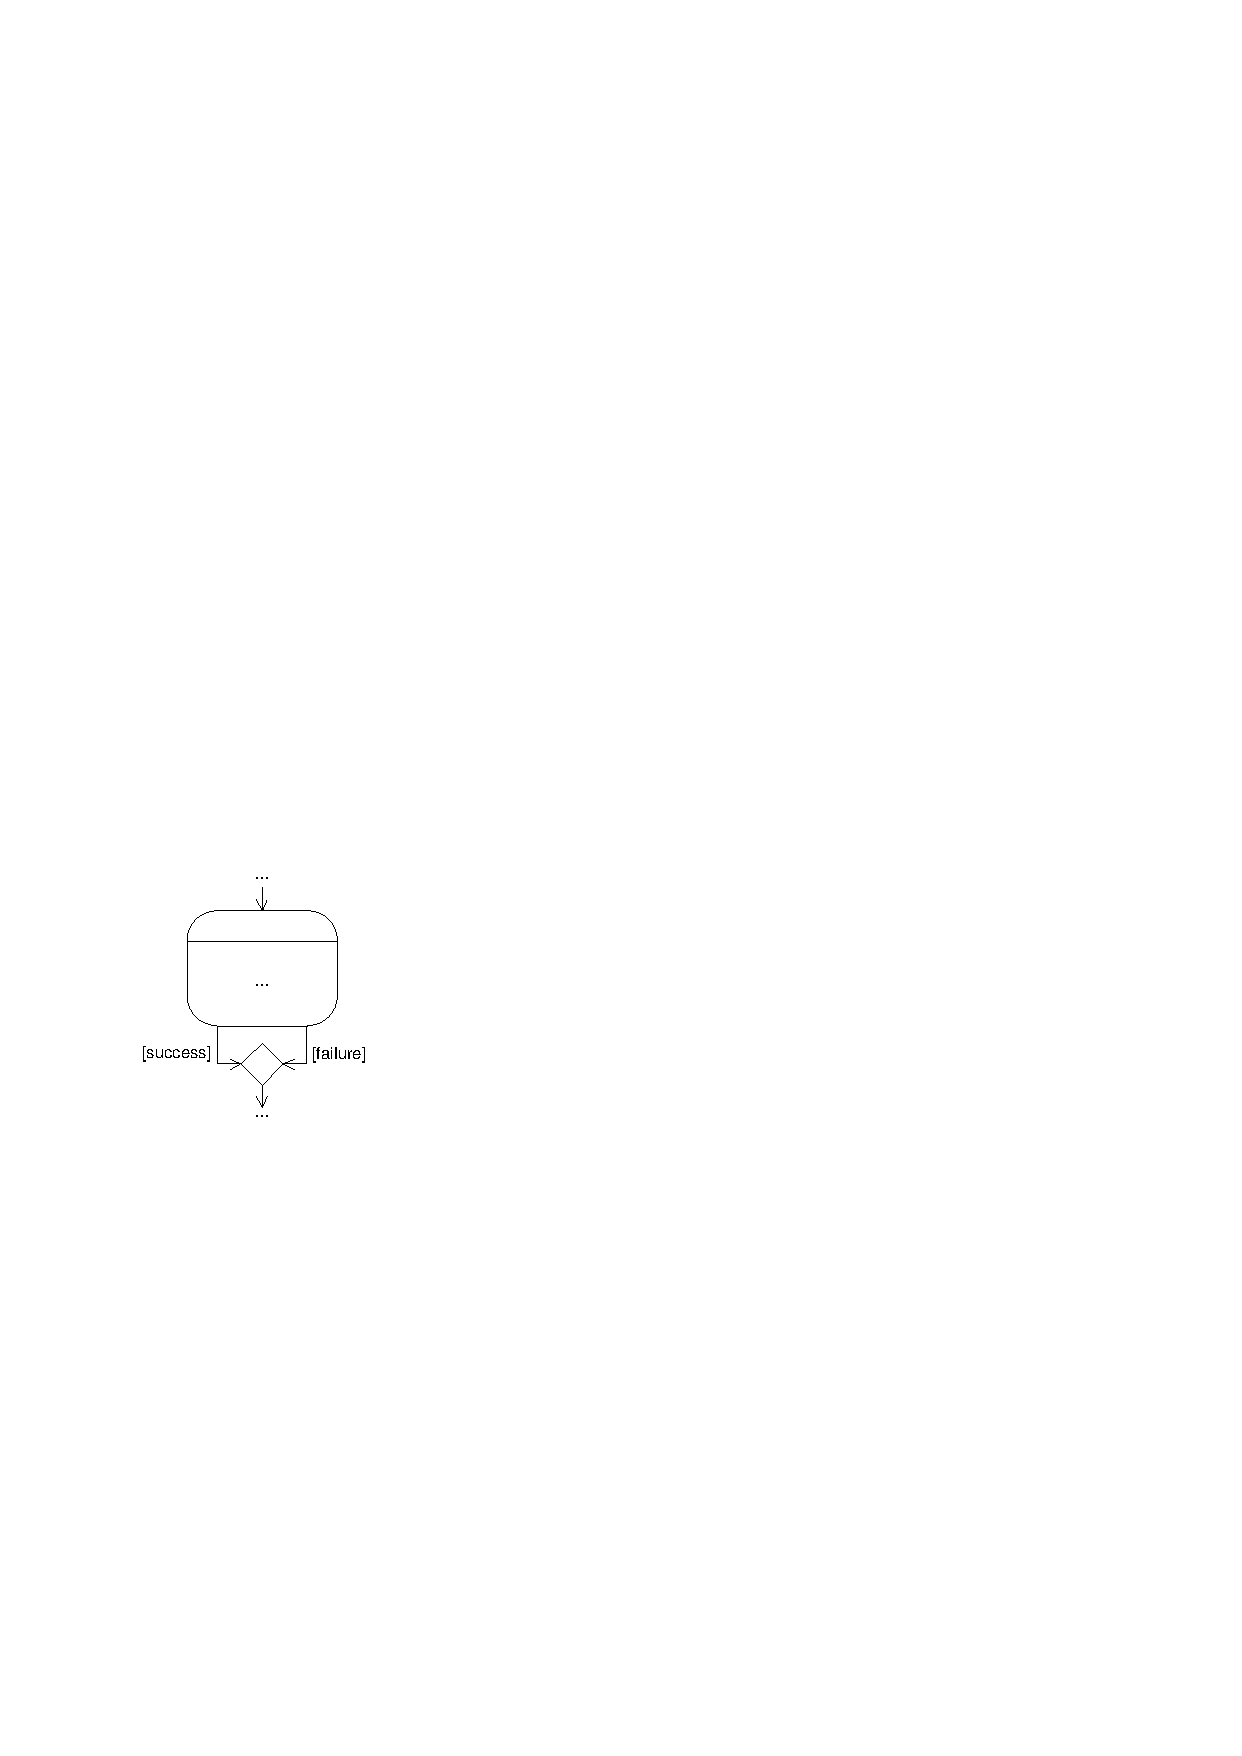
\includegraphics[scale=0.9]{SD-simplify1a} 
    \\a)
    %\caption{a) Each-Time Loop}
    %\label{fig:SD-loop-for-each}
  \end{minipage}%
  \hfill
  \begin{minipage}[t]{.24\textwidth}
    \centering
    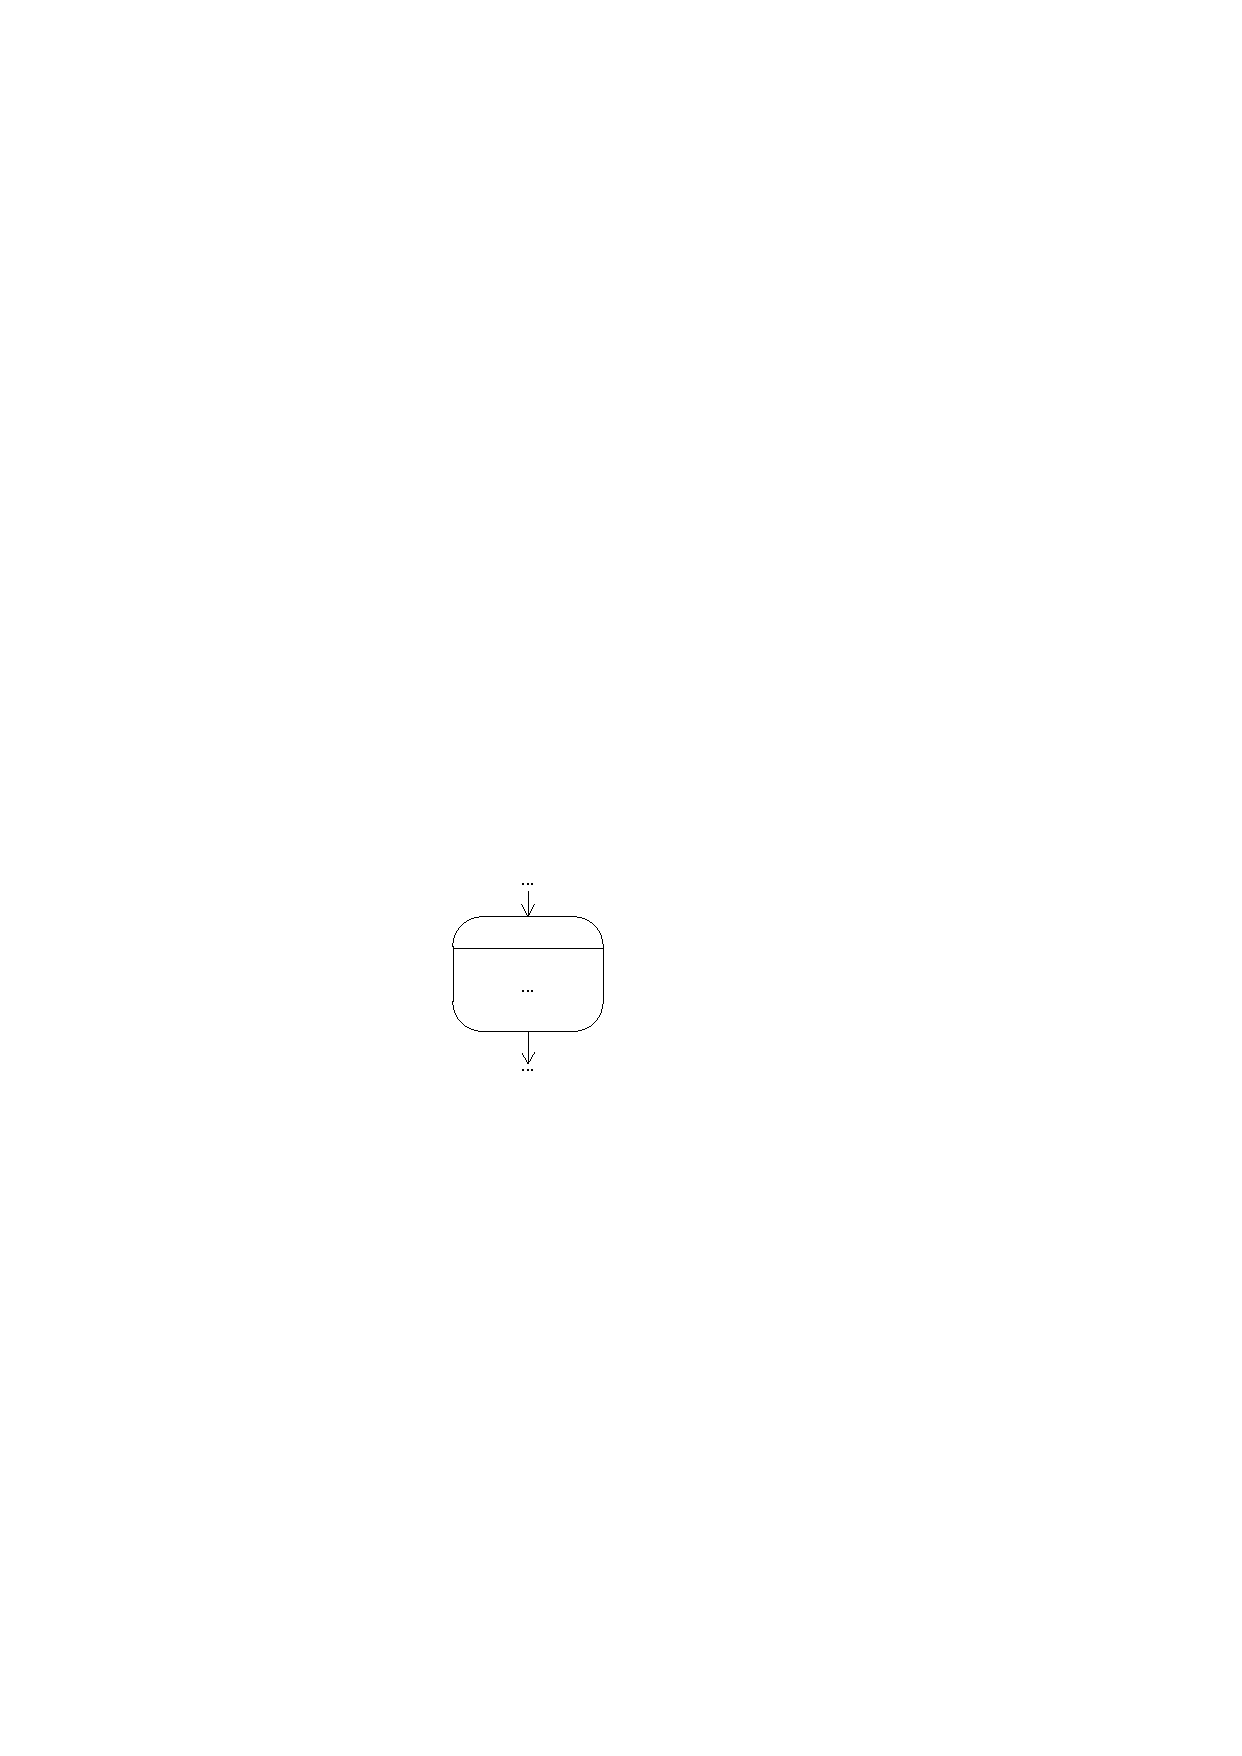
\includegraphics[scale=0.9]{SD-simplify1b}
    \\b)
    %\caption{b) Matching-Dependent Loop}
    %\label{fig:SD-loop-matching}
  \end{minipage}
  \hfill
  \begin{minipage}[t]{.24\textwidth}
    \centering
    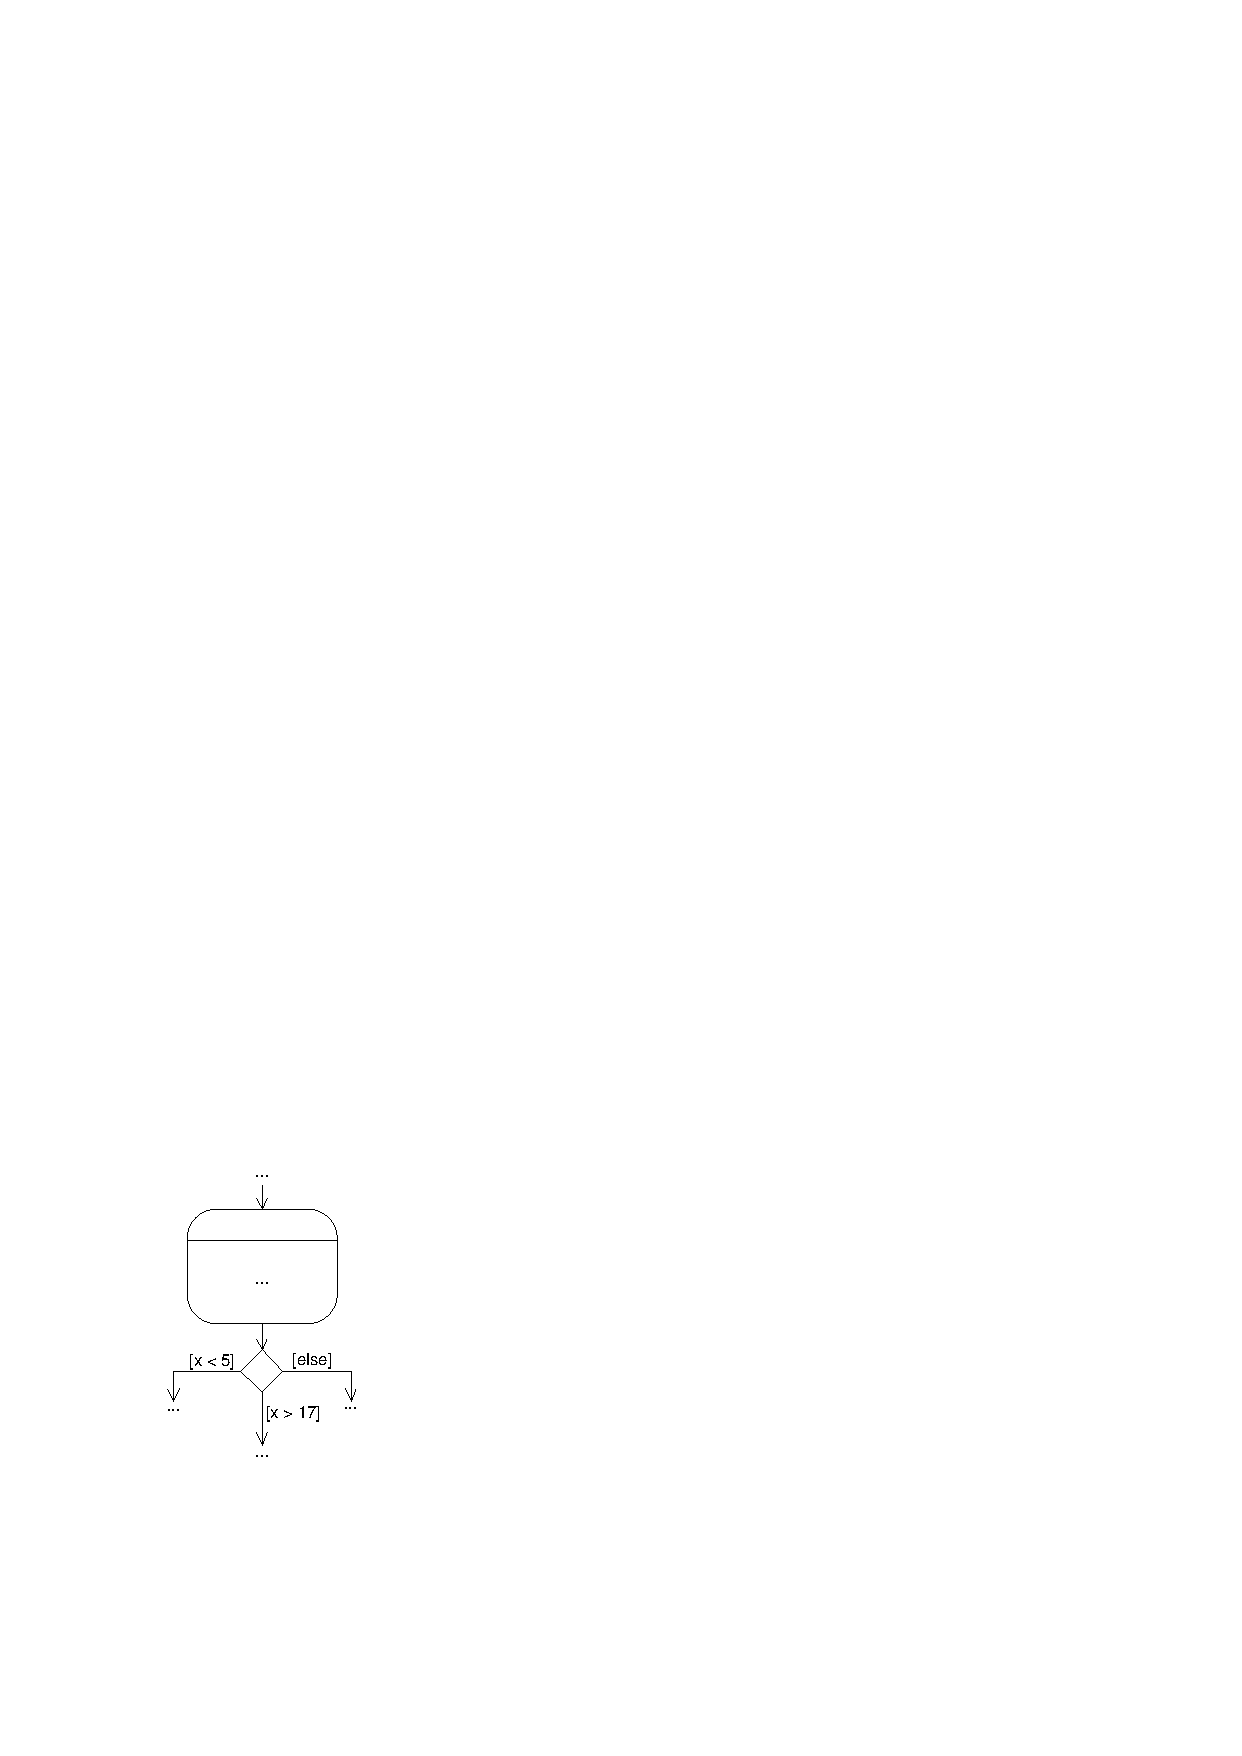
\includegraphics[scale=0.9]{SD-simplify2a}
    \\c)
    %\caption{c) Boolean-Condition Loop}
    %\label{fig:SD-loop-boolean}
  \end{minipage}
  \hfill
  \begin{minipage}[t]{.24\textwidth}
    \centering
    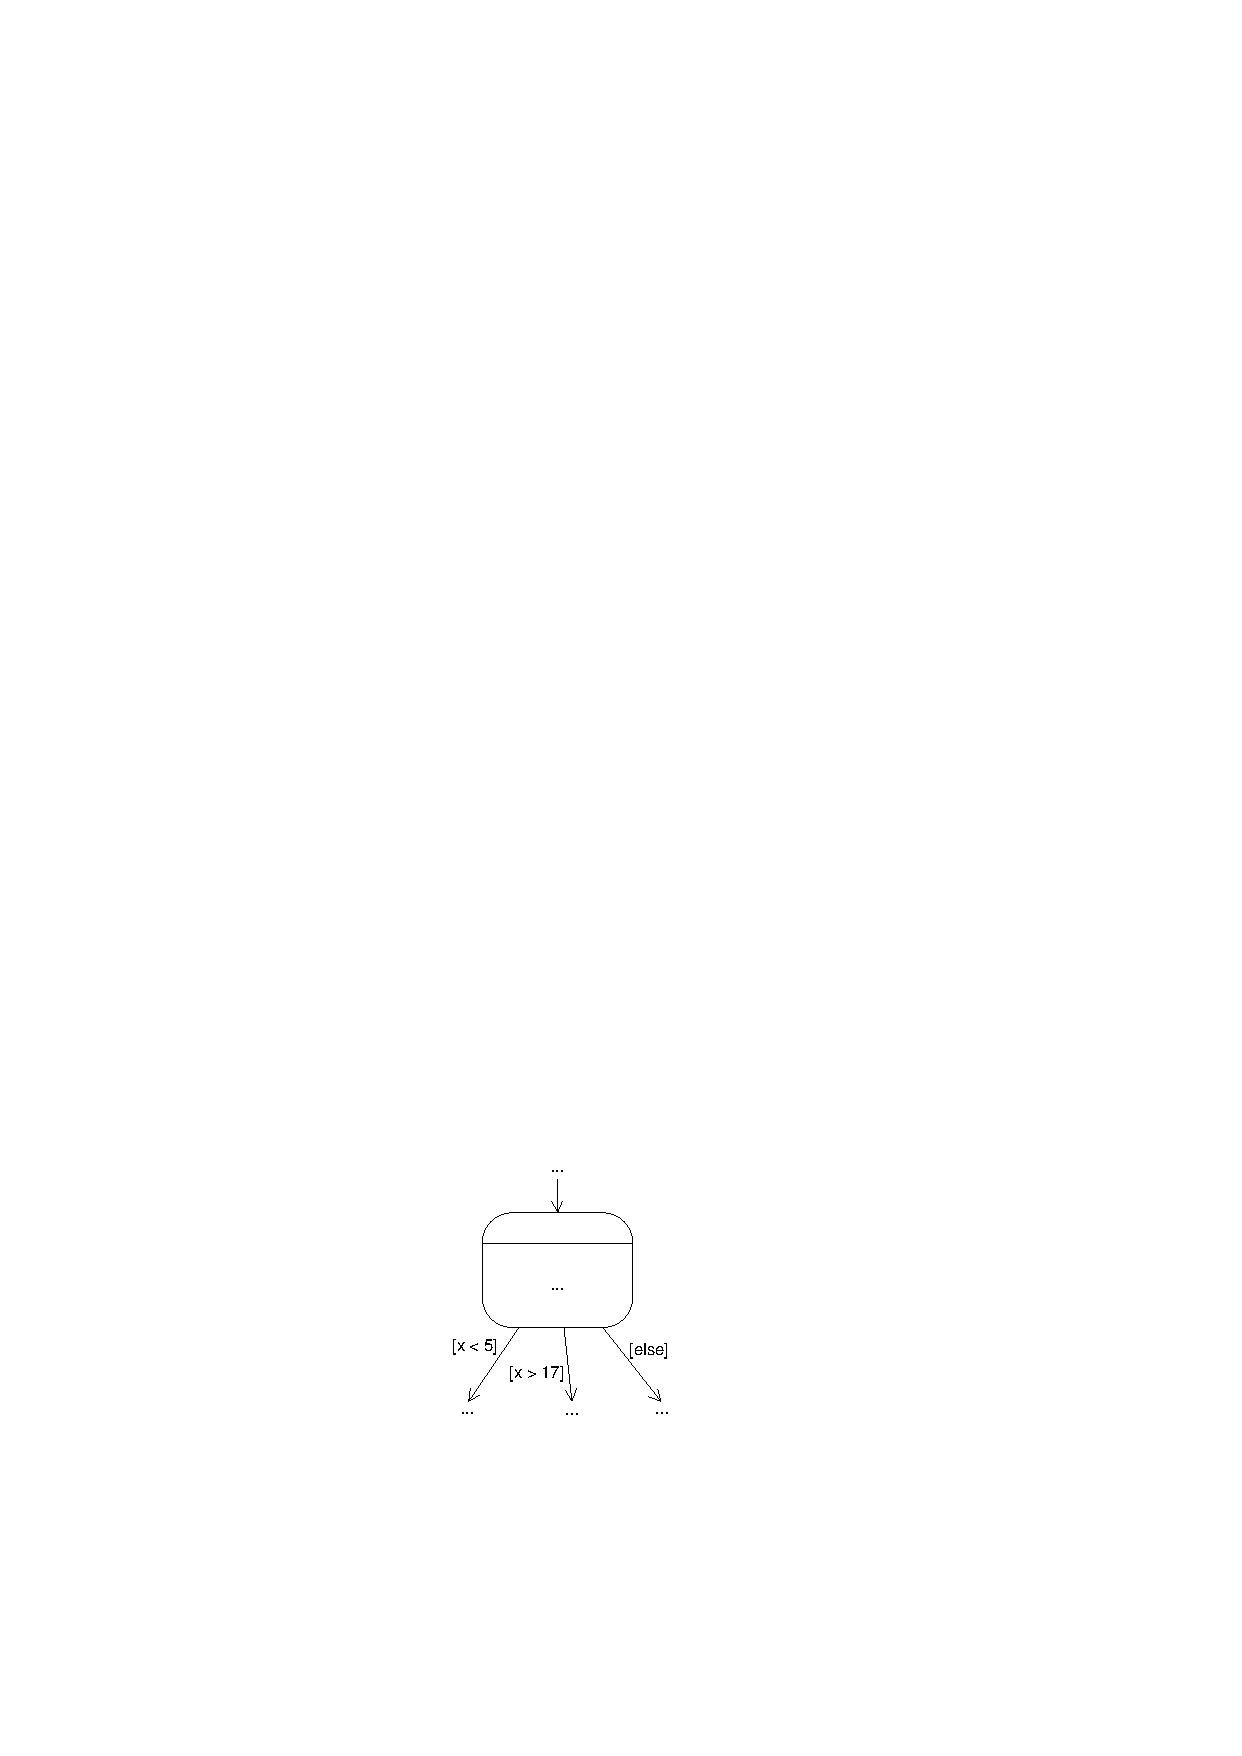
\includegraphics[scale=0.9]{SD-simplify2b}
    \\d)
    %\caption{c) Boolean-Condition Loop}
    %\label{fig:SD-loop-boolean}
  \end{minipage}
  \caption[Examples For Control Flow Simplifications]{Examples For Control Flow Simplifications: case a) is semantically equivalent to b), case c) is semantically equivalent to d)}
  \label{fig:SD-simplifications}
\end{figure}

The junction node can also be used to merge several control flows into one
(several activity edges point to a junction node which has only one outgoing activity edge,
see Figure~\ref{fig:SD-simplifications} a)).

In order to simplify the control flow as shown in Figures~\ref{fig:SD-simplifications} a) and c),
we also allow shorthand notations as illustrated in Figures~\ref{fig:SD-simplifications} b) and d).
The control flow in case b) is semantically equivalent to that in case a).
The control flows in cases c) and d) are also equivalent.

\begin{figure}[htb]
	\centering
  \begin{minipage}[t]{.3\textwidth}
    \centering
    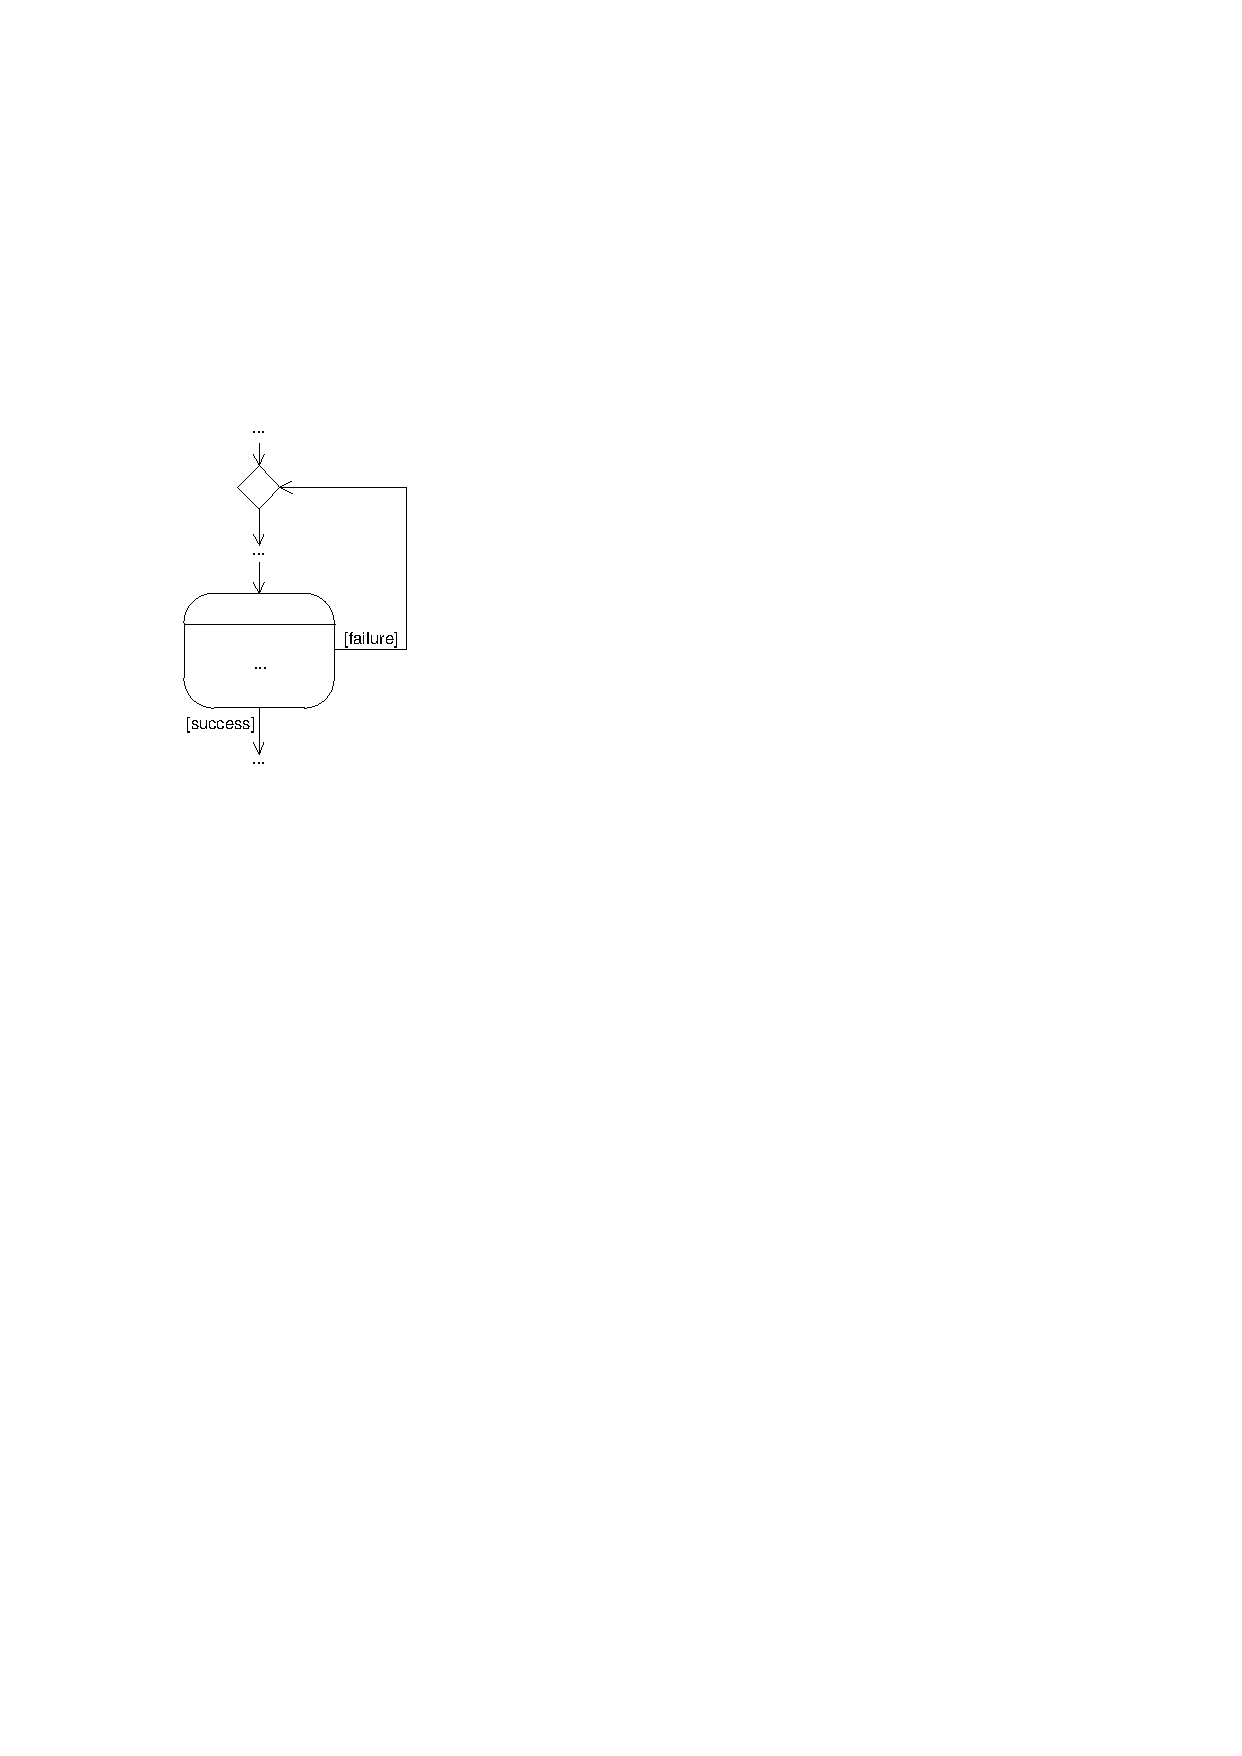
\includegraphics[scale=1]{SD-loop1} 
    \\a)
    %\caption{a) Each-Time Loop}
    %\label{fig:SD-loop-for-each}
  \end{minipage}%
  \hfill
  \begin{minipage}[t]{.3\textwidth}
    \centering
    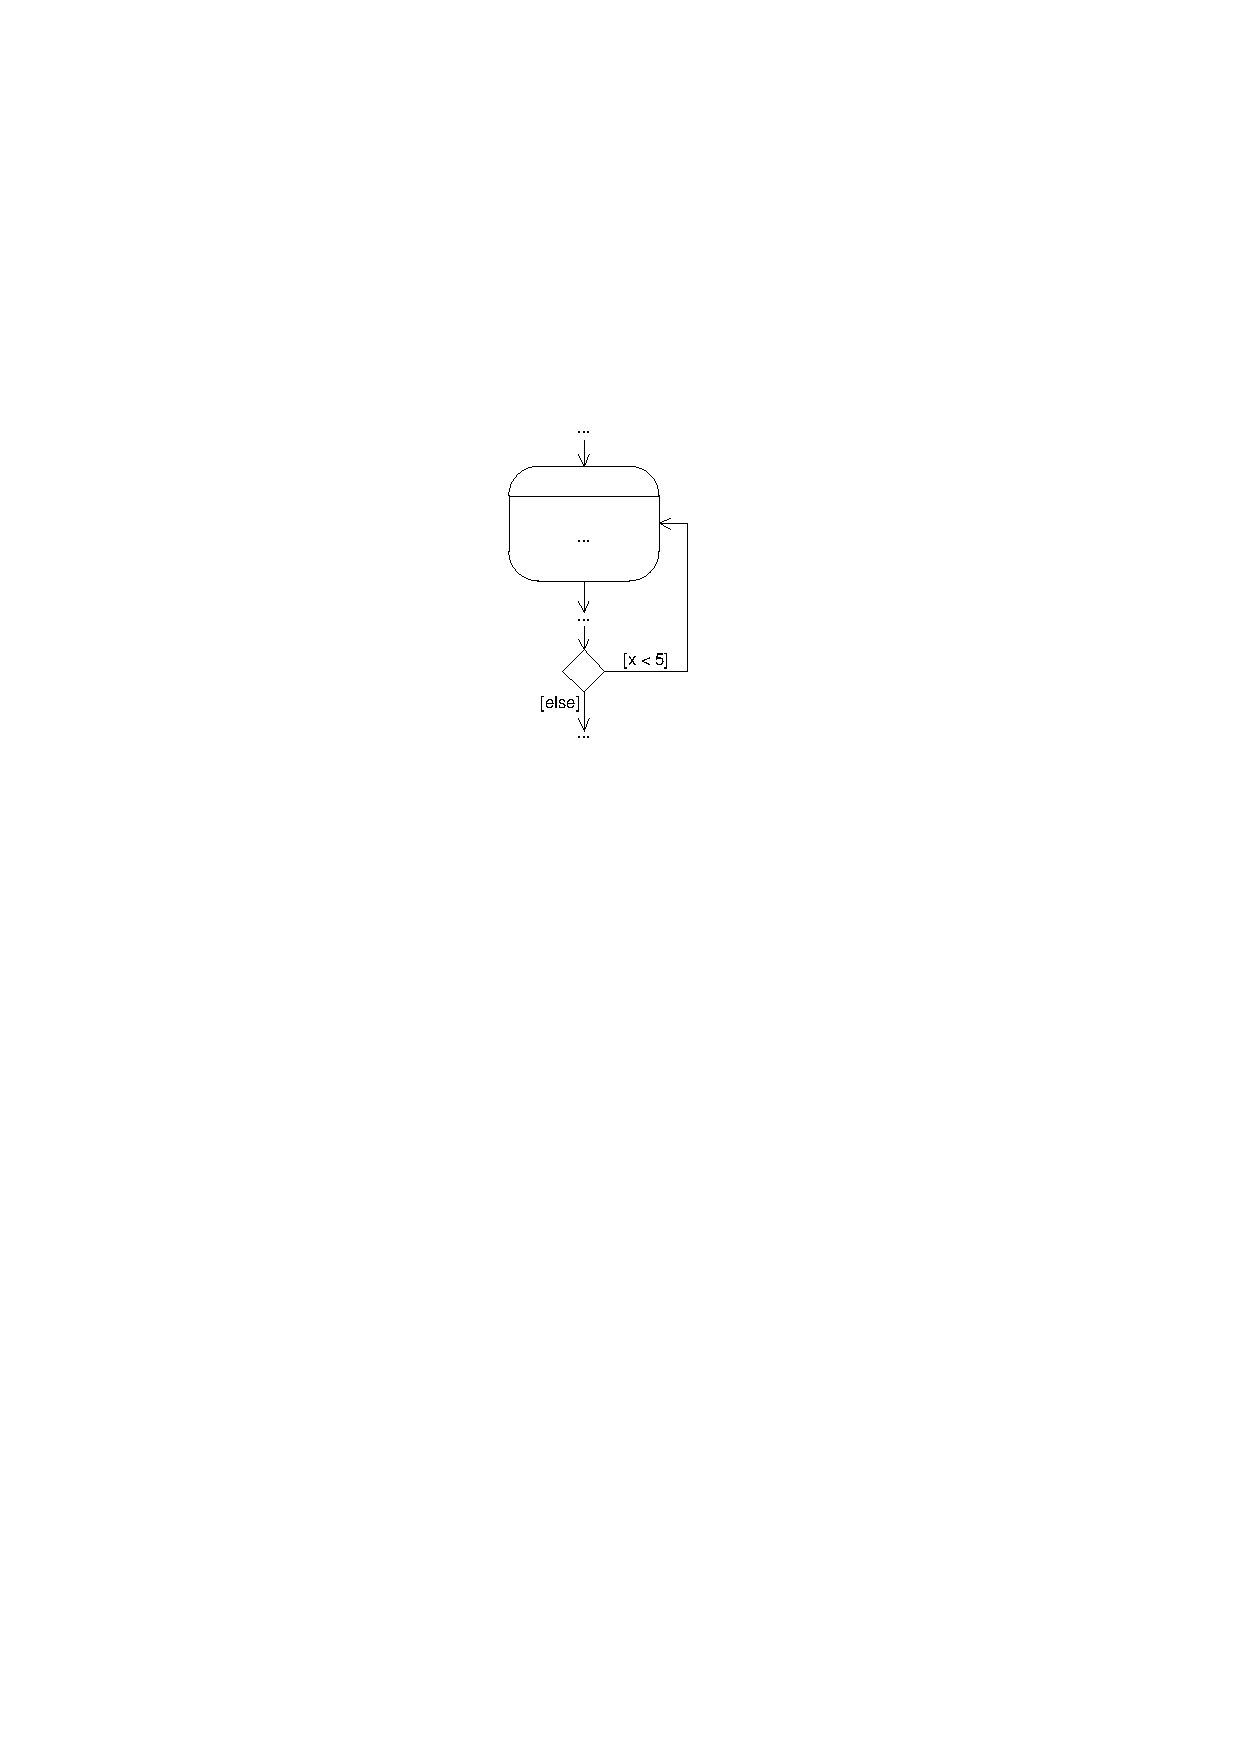
\includegraphics[scale=1]{SD-loop2}
    \\b)
    %\caption{b) Matching-Dependent Loop}
    %\label{fig:SD-loop-matching}
  \end{minipage}
  \hfill
  \begin{minipage}[t]{.3\textwidth}
    \centering
    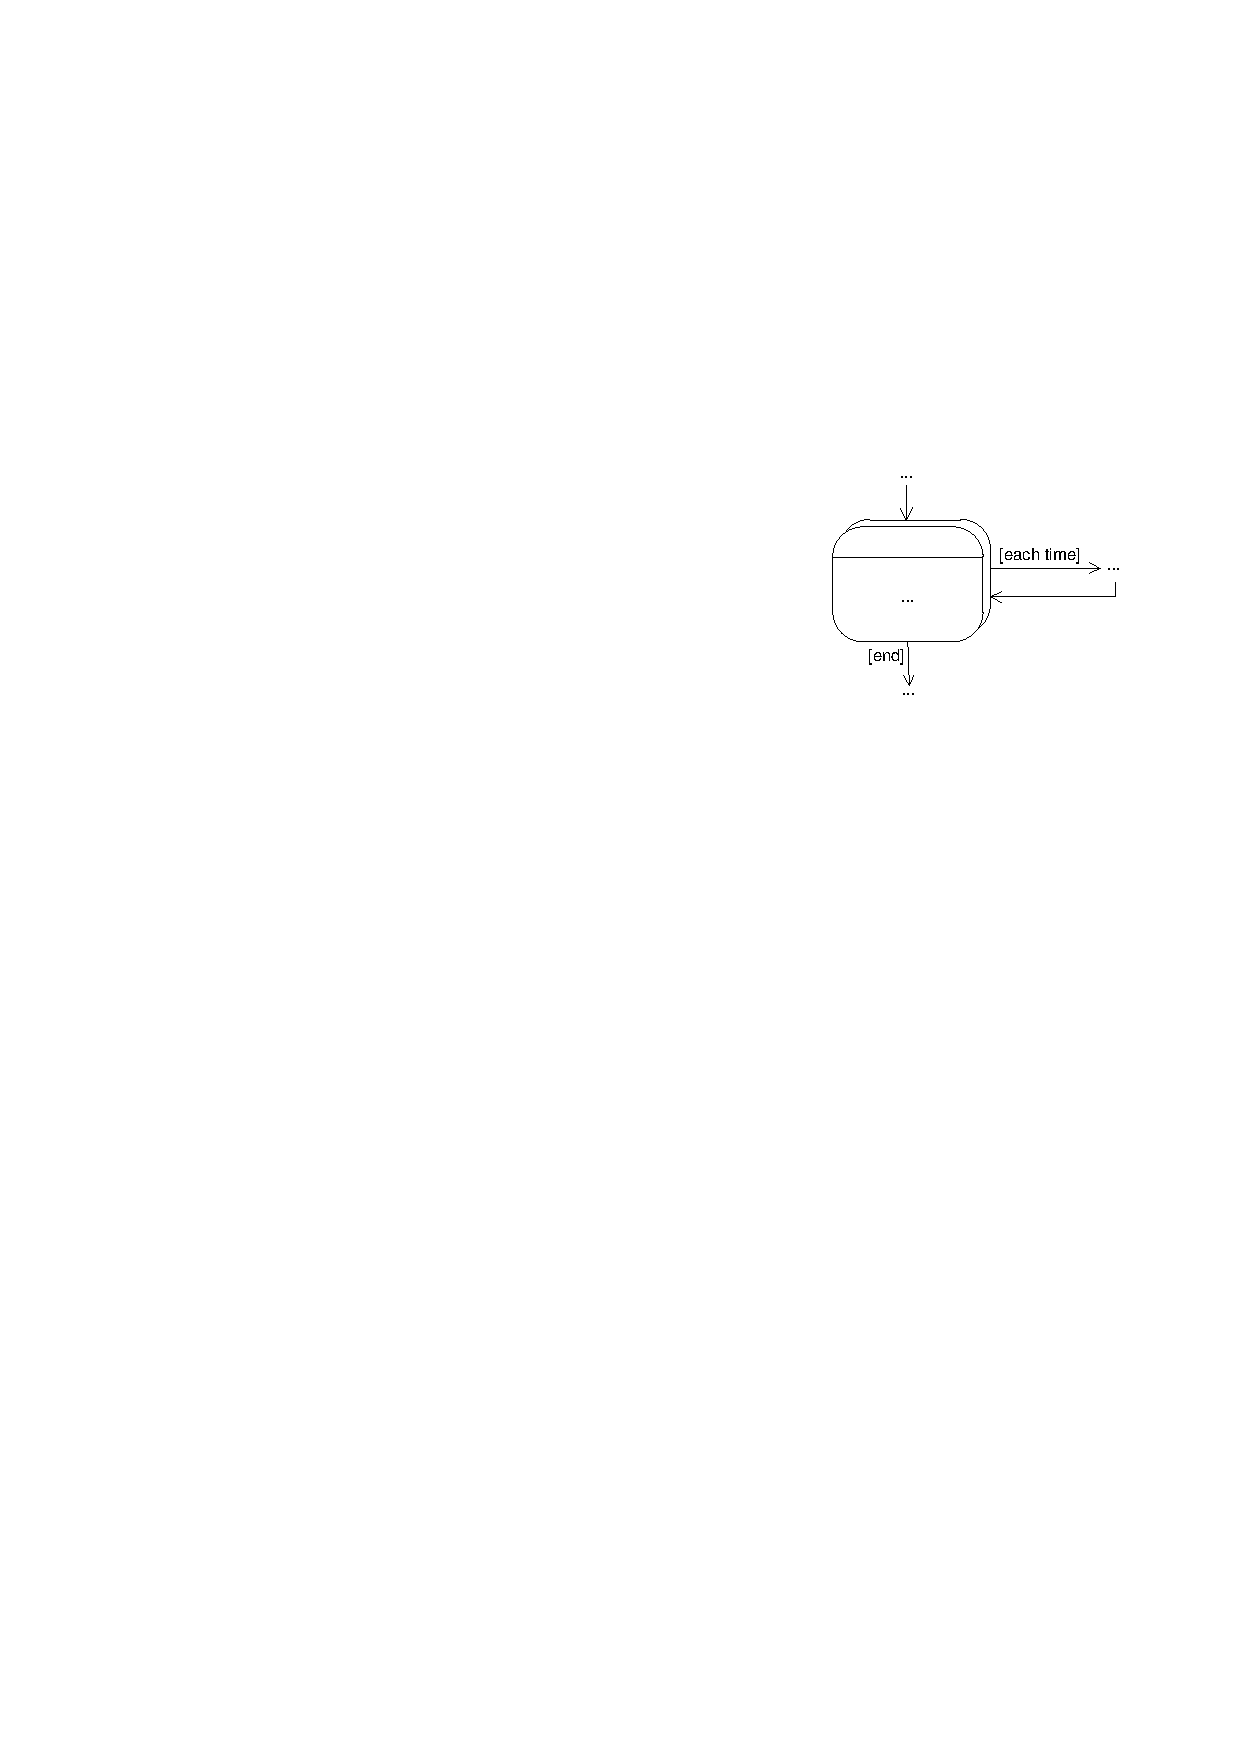
\includegraphics[scale=1]{SD-loop3}
    \\c)
    %\caption{c) Boolean-Condition Loop}
    %\label{fig:SD-loop-boolean}
  \end{minipage}
  \caption{Examples For Loops}
  \label{fig:SD-loops}
\end{figure}

Activity edges and guards can be used to model loops as illustrated in Figures~\ref{fig:SD-loops} a) and b).
There is an additional construct to model loops which allows to perform the same operations with each occurrence of a certain object structure.
For that purpose, we use a special activity node that we call \emph{for-each} activity node
and special guards \fe{\text[each time\text]} and \fe{\text[end\text]}.

The for-each activity node is depicted by a cascaded activity node (see Figure~\ref{fig:SD-loops} c)).
The second activity node in Figure~\ref{fig:simpleStoryDiagram} (p.~\pageref{fig:simpleStoryDiagram}), for example, is a for-each activity node.
Such a node represents a loop where the contained story pattern is executed as often as new subgraphs can be matched
that differ from the previously matched graphs by at least one other matched object.
The story pattern in the for-each activity node in Figure~\ref{fig:simpleStoryDiagram}
is matched for each existing pair of a method (object variable \fe{anyMethod}) and corresponding call object (object variable \fe{c}).
Besides the matching itself, all \emph{destroy} and \emph{create} steps are also executed for each of these matched subgraphs.
In general, after execution of the story pattern in the for-each activity node,
the control flow follows the activity edge with the guard \fe{\text[each time\text]}, if available (see Figure~\ref{fig:SD-loops} c)).
This edge is optional and can be omitted like in Figure~\ref{fig:simpleStoryDiagram}.
The \fe{[each time]} edge leads to the activity node (or a sequence of such nodes)
that is to be executed after each successful execution of the for-each activity node.
After that, the control flow returns to the for-each activity node in order to match and process the next object structure that can be matched by the for-each activity node.
If there is an activity edge with the guard \fe{\text[each time\text]}, there has also to be such an activity edge leading back to the for-each activity node.
This constitutes a loop.
Finally, the control flow is guided by the activity edge with the guard \fe{\text[end\text]} which leads to the activity node to be executed after the loop.
Each for-each activity node must have such an outgoing \text[end\text] activity edge.

\todojr{fresh matches, auch fuer maybe\_bound: Behaelt ein maybe\_bound-Knoten ein Binding, was erst im Loop gesetzt wurde? Oder zaehlt dafuer nur, was vor dem Loop schon gebunden war? Letzteres erscheint sinnvoller (Stephan fragen wegen Beispiel)}

\subsection{Propagation of Matchings}
\label{sec:storydiagrams:propagation}

The control flow specified by the activity edges determines how matchings of story patterns are propagated through the story diagram. An initial matching associating objects of the instance model with object variables is established by the input parameters of the story diagram. In a story pattern inside a story node, we refer to matched objects by using bound variables. Then, the story pattern inside a story node is matched. If the matching process was successful, the matching is extended by the objects which were newly matched by the story pattern and is propagated via the \emph{success} activity edge to the next activity node. If the matching process was not successful, the matching is not changed and the original matching which was passed to the activity node is propagated along the \emph{failure} activity edge. The matching process includes both, the matching step and the modification step. If a match could be obtained, but the modification step fails, e.g. due to unsatisfiable link constraints (cf. Section~\ref{sec:StoryPatterns:linkConstraints}), the story pattern is also considered to be failed and the story node is left via the \emph{failure} activity edge. If a story pattern failed, it also does not change the instance model.

In case of a loop, the matching which is propagated into the for-each activity node is extended by the matching of the story pattern which is contained in this activity node. If the matching is successful, the extended matching is propagated along the \emph{each time} activity edge. The matching may then be extended and changed by the subsequent activity nodes forming the loop body. If the control flow returns to the for-each activity node, the matching needs to be restricted to the object variables that were initially passed to the for-each activity node. That has two basic consequences. First, if a variable which was part of the matching that was initially provided to the for-each activity node has been changed to another object, that change is preserved for the next iteration. Second, if a variable which was not part of the matching that was initially provided to the for-each activity node has been bound in the loop, it is removed from the matching for the next iteration. As a result, the matching which is propagated down the \emph{end} activity edge only contains those object variables which were initially passed to the for-each activity node. The object variables, however, may be bound to different objects after executing the loop. Objects and links created throughout the loop remain in instance model although the object variables they were bound to are no longer visible in the matching. That semantics corresponds to the semantics of loops in programming languages as, e.g., Java. 

\begin{figure}[htbp]
\begin{center}
  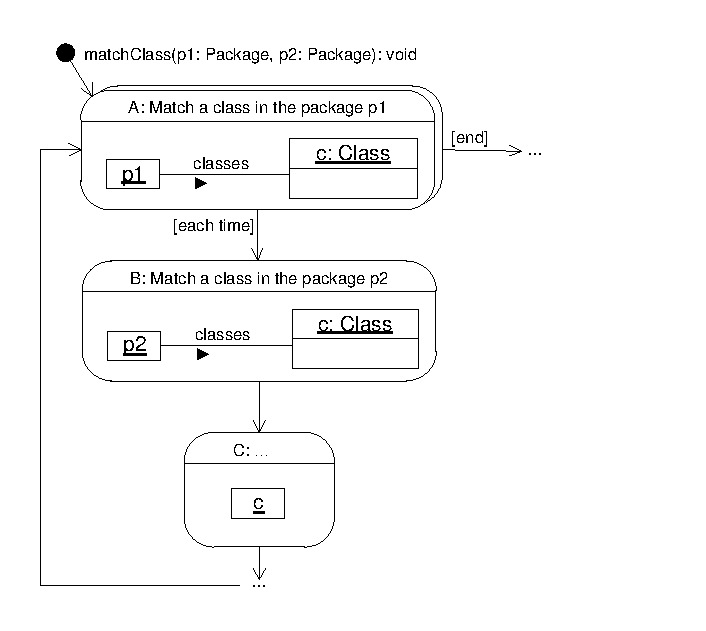
\includegraphics[scale=1.0]{figures/PropagationOfMatchingsExample}
  \caption{Propagation of Matchings through a Story Diagram}
  \label{fig:propagation}
\end{center}
\end{figure}

Figure~\ref{fig:propagation} gives an example for the propagation of matchings. The initial matching consists of two objects of type \fe{Package} which are bound to the input parameters \fe{p1} and \fe{p2}. This matching is passed to the for-each activity node \fe{A}. In this activity node, the story pattern tries to match a class in the package bound to \fe{c}. For each class that is found, the matching is extended by the corresponding class and propagated along the \emph{each time} activity edge to the activity node \fe{B}. In \fe{B}, the object variable \fe{c} is unbound. Thus, a new matching for \fe{c} is to be obtained. If the story pattern is matched successfully, the matching that is propagated down the activity edge to \fe{C} consists of the two packages as well as a class contained in the package bound to \fe{p2}. If the story pattern in \fe{B} cannot be matched, then the matching is propagated unchanged. Then the matching in \fe{C} contains the two packages as well as a class which is contained in the package bound to \fe{p1}. If the control flow reaches the for-each activity node \fe{A} again, then the matching is reduced to the object variables \fe{p1} and \fe{p2} because they constituted the matching initially propagated in \fe{A}. If \fe{p1} or \fe{p2} were bound to a new object during the loop  body, that change would be preserved and the new objects bound to \fe{p1} or \fe{p2} are used in the next iteration. The object variable \fe{c} is removed from the matching and may not be used for the next iteration.

If the control flow reaches a final node, only objects that are contained in the matching which is propagated to the final node may be returned. The use of decision nodes in combination with activity edges having a boolean guard does not change the propagation of matchings. The boolean condition at the edge only defines where the matching is propagated.

\subsection{Story Diagram Calls}
\label{sec:Calls}
Story diagram calls are special nodes in a story diagram which are used to invoke other story diagrams. Similar to method calls, this reduces redundancy and promotes reuse.

As described in Section~\ref{sec:activities}, a story diagram can have an arbitrary number of in and out parameters. When calling a story diagram, concrete arguments have to be assigned to the in parameters. Consequently, if an object variable named \fe{n} is bound somewhere in the story diagram, the identifier \fe{n} can be used to pass this object variable as an argument to a call. If the called story diagram has out parameters, those are bound explicitly by assignments at the stop activity node. They can be used in the calling story diagram by specifying object variables whose names match those of the out parameters.

For in parameters, we use a call-by-reference semantics. If an object that is passed as an in parameter is modified in the called story diagram, those modifications remain after the called story diagram has terminated. The object in question can be used in the calling story diagram after the call but the call may have modified its attributes or its links.

An example of a story diagram call is shown in Figure~\ref{fig:call}.

\begin{figure}[htb]
\begin{center}
  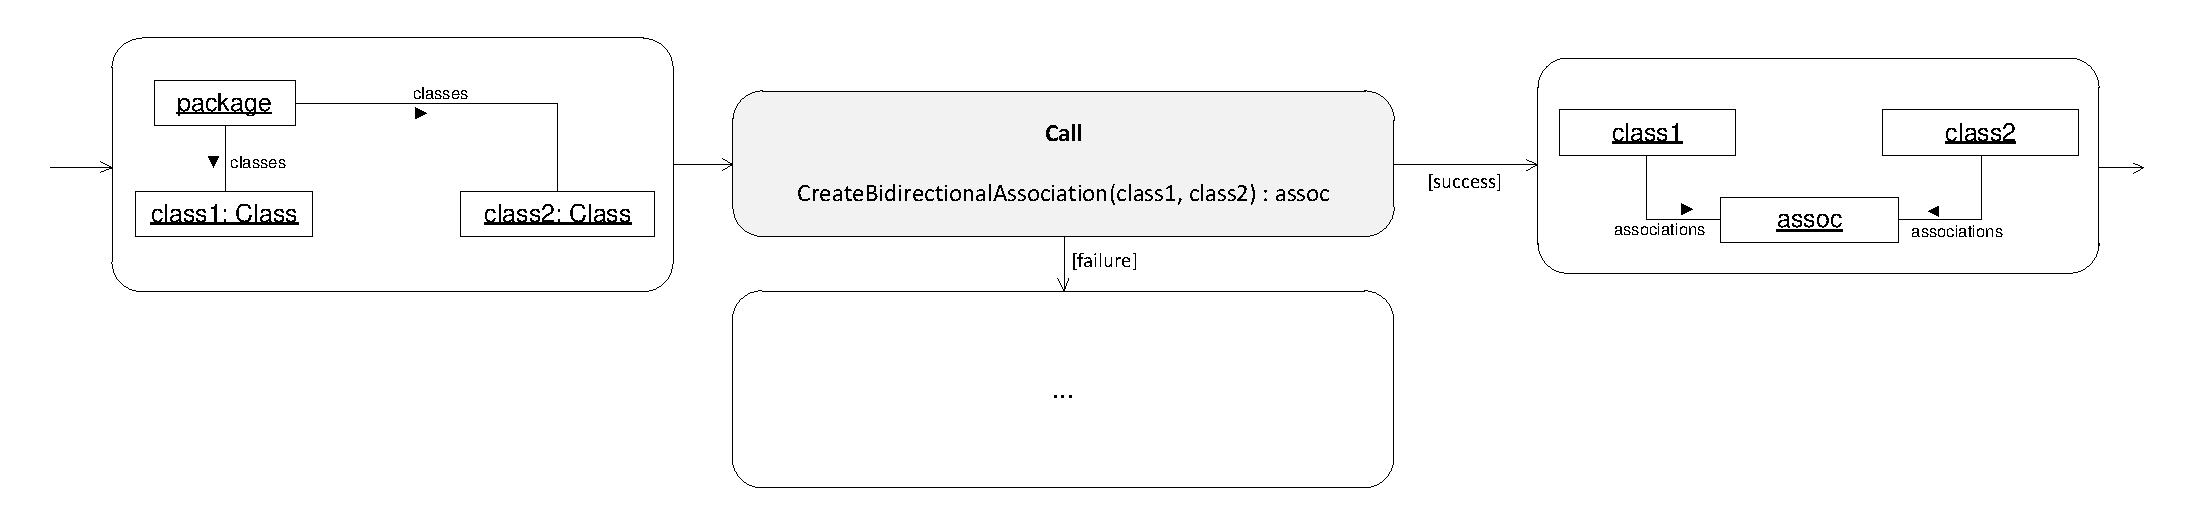
\includegraphics[width=\textwidth]{figures/StoryDiagramCall}
  \caption{Example of a story diagram call}
  \label{fig:call}
\end{center}
\end{figure}

The first story pattern in Figure~\ref{fig:call} shows the bound object variable \fe{package}. Two new object variables \fe{class1} and \fe{class2} are bound in that pattern. The next node with the grey background is a story diagram call which is also signified by its label \fe{Call}. Beneath the label, the name of the called story diagram is given, in this case \fe{CreateBidirectionalAssociation}. Assume that the called story diagram has two in parameters of the type \fe{Class} and one out parameter of the type \fe{Association}. The two classes that were bound in the first story pattern, \fe{class1} and \fe{class2} are passed to the call as arguments. They can be used in the story node after the call without passing the back as out parameters. The modifications carried out by the called story diagram (i.e.\ the creation of the \fe{assoc} object and its connection to \fe{class1} and \fe{class2}) are retained after the call terminates.
The result of the call is bound to the object variable \fe{assoc}. The type of this variable is determined by the out parameter type, i.e., in this case the type Association.

If a story diagram has no out parameters, the keyword \fe{void} follows the colon instead of the out parameter's names (see Figure \ref{fig:SDRemoveInterfaceViolation} for an example).

%Issues for future versions:
% method calls
% polymorphic calls

%\ext
{
\subsection{Exception Handling}
}


